\documentclass[11pt,a4paper]{article}
\usepackage[utf8]{inputenc}
\usepackage{amsmath}
\usepackage{mathtools}
\usepackage{amsfonts}
\usepackage{amssymb}
\usepackage{graphicx}
\usepackage{caption}
\usepackage{subcaption}
\usepackage{comment}
\usepackage{color}
\usepackage{enumitem}
\usepackage[left=2cm,right=2cm,top=2cm,bottom=2cm]{geometry}
\usepackage{listings}
\usepackage{color}

\setlength{\jot}{10pt}
 
\definecolor{codegreen}{rgb}{0,0.6,0}
\definecolor{codegray}{rgb}{0.5,0.5,0.5}
\definecolor{codepurple}{rgb}{0.58,0,0.82}
\definecolor{backcolour}{rgb}{0.95,0.95,0.92}
 
\lstdefinestyle{mystyle}{
    backgroundcolor=\color{backcolour},   
    commentstyle=\color{codegreen},
    keywordstyle=\color{magenta},
    numberstyle=\tiny\color{codegray},
    stringstyle=\color{codepurple},
    basicstyle=\footnotesize,
    breakatwhitespace=false,         
    breaklines=true,                 
    captionpos=b,                    
    keepspaces=true,                 
    numbers=left,                    
    numbersep=5pt,                  
    showspaces=false,                
    showstringspaces=false,
    showtabs=false,                  
    tabsize=2
}
 
\lstset{style=mystyle}
\graphicspath{ {./figs/} }
\author{Andrew Teta}
\title{ECEN 4532 - Lab 1: Sound Processing in Python}

\begin{document}

\maketitle
\begin{figure}[ht]
	\centering
	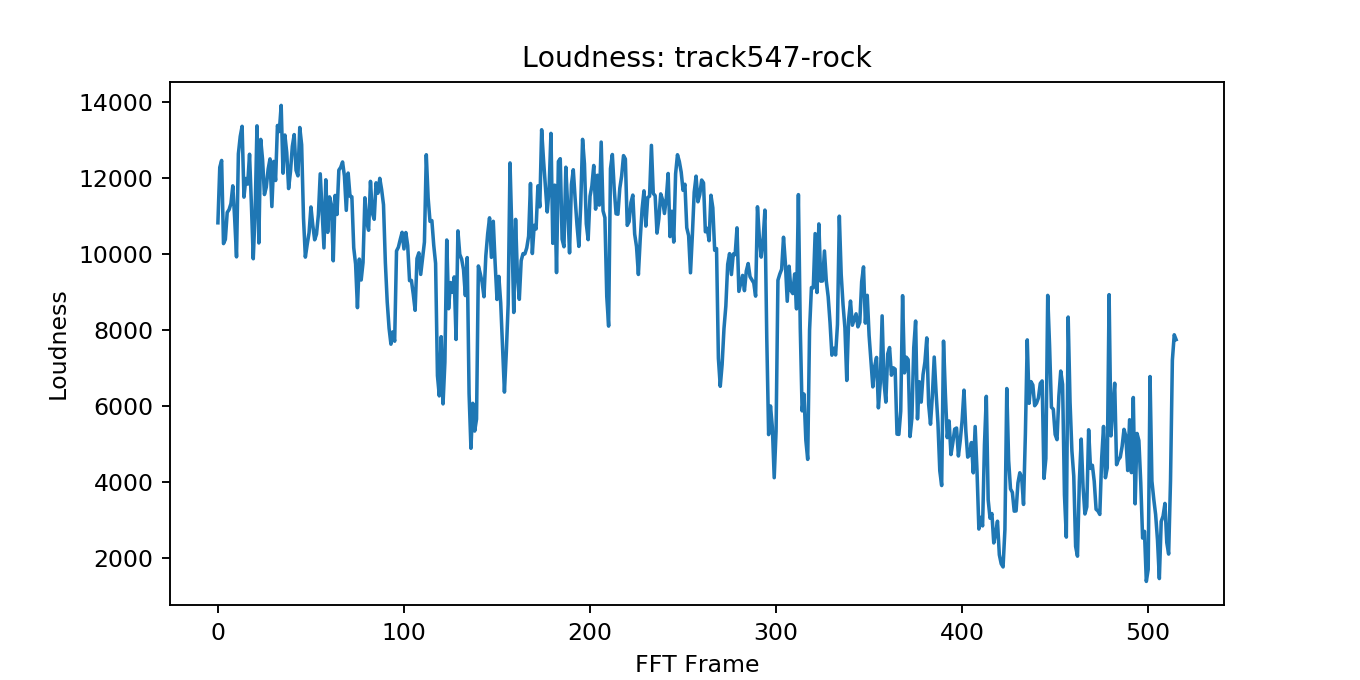
\includegraphics[width=0.9\textwidth]{loudness_track547-rock}
\end{figure}

\pagebreak

\tableofcontents

\pagebreak

\addcontentsline{toc}{section}{Introduction}
\section*{Introduction}
\paragraph*{} In this discussion, we will be exploring some techniques recently developed in the audio industry to organize, search, and classify large music collections. We are developing some statistical methods, along with frequency analysis to automatically characterize songs and genres.
\addcontentsline{toc}{subsection}{Format}
\subsection{Background}
\paragraph*{} Fundamentally, we begin with a '.wav' file. This is one variety of many signal encodings, generated by sampling a physical sound wave using a microphone. The microphone detects pressure differences within a medium (sound) and converts them into electrical voltages. As the voltages are converted into a digital representation, they are quantized at a sampling frequency ($fs$). Furthermore, the Nyquist sampling theorem dictates that for a signal to be represented accurately in quantized form, it must be sampled at twice the rate of the highest frequency component. For example, a dolphin can only hear sound in the range $7kHz-120kHz$, so if we want to record the sound that a dolphin would be able to hear, we have to sample at a rate $fs=240kHz$ or higher.
\paragraph*{} In this lab, we consider a small collection of music, organized by genre, in '.wav' format. Each song is sampled at $fs=11,025Hz$. Narrowing our data set even further, we will extract a 24 second sample from the middle of each song. We will then implement a short-time Fourier transform (STFT), which divides the sample into $N=512$ samples, or $46ms$ and call each 46 ms interval a 'frame'. The STFT is a good way to obtain frequency spectrum data, while maintaining a level of time-domain relevance. For the purposes of this lab, the frames will be non-overlapping.

\section{Time-domain Analysis}
\paragraph*{} We begin by extracting a $24s$ sample from the middle of each song using the python function \verb|scipy.io.wavfile.read|. See section \ref{app:timedomain} for Python implementation.
\subsection{Loudness}
\paragraph{} To get a sense of 'loudness', we will compute the standard deviation over a 'frame' of size $N=512$ defined as:

\begin{align}
\sigma(n)=\sqrt{\frac{1}{N}\sum_{m=0}^{N-1} [x(nN+m)-E[x_n]]^2} && \text{with} && E[x_n]=\frac{1}{N}\sum_{m=0}^{N-1} x(nN+m)
\end{align}

See section \ref{app:loudness} for Python implementation.

\paragraph{Results} The output of the loudness calculation for one song of each genre is shown in the figures below. 

\begin{figure}[tb]
	\centering
	\begin{subfigure}[t]{\hsize}
		\centering
		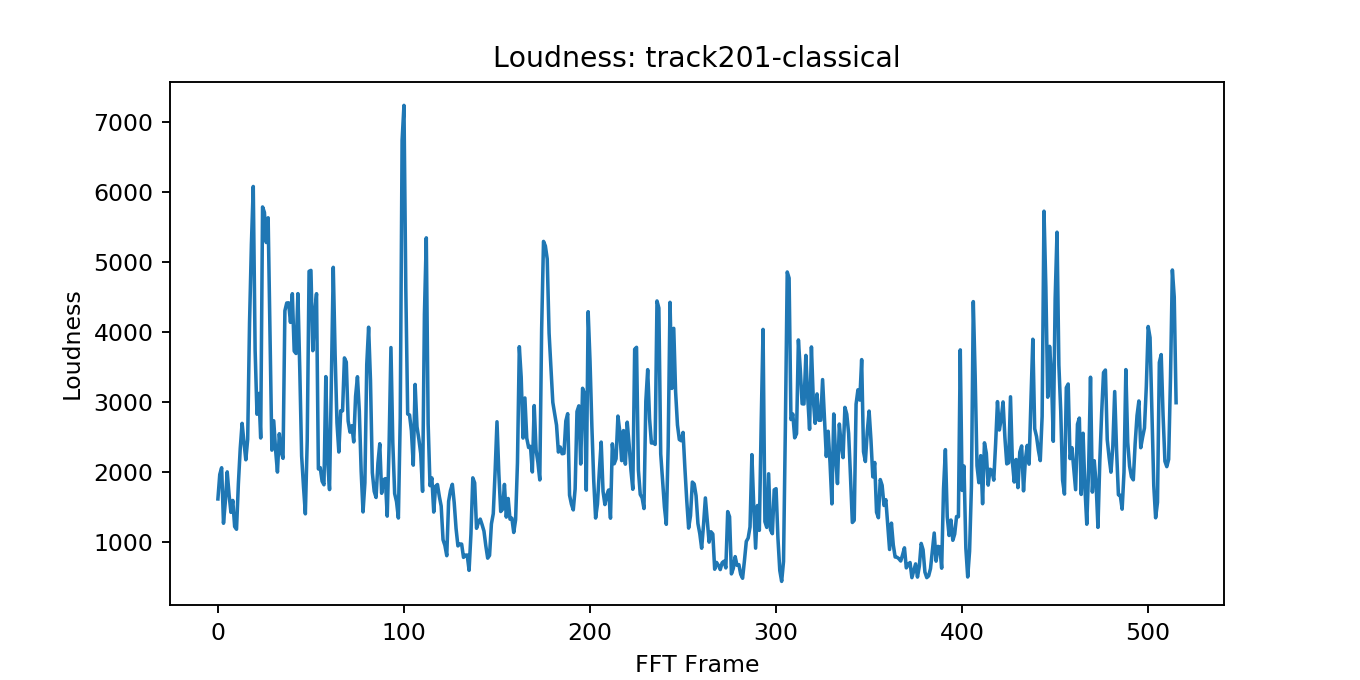
\includegraphics[width=0.9\textwidth]{loudness_track201-classical}
		\caption{'track201-classical.wav'}
		\label{fig:loudness_classical}
	\end{subfigure}
	\begin{subfigure}[t]{\hsize}
		\centering
		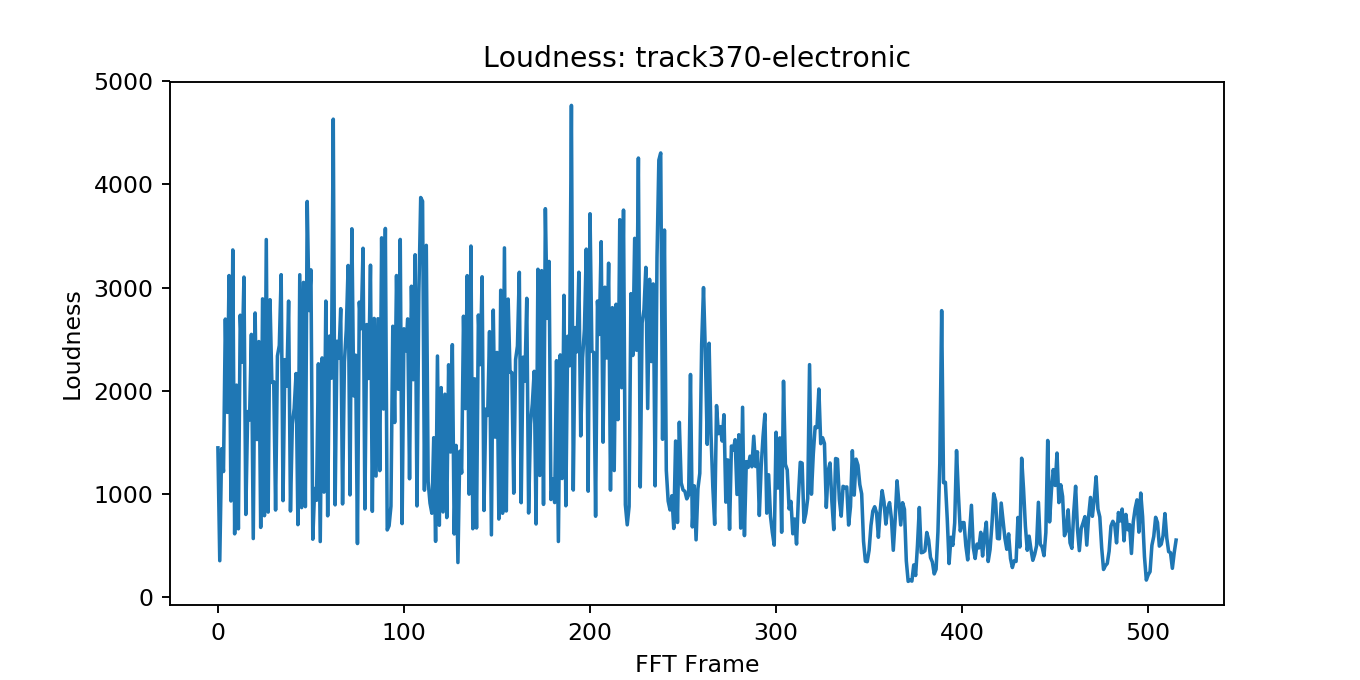
\includegraphics[width=0.9\textwidth]{loudness_track370-electronic}
		\caption{'track370-electronic.wav'}
		\label{fig:loudness_electronic}
	\end{subfigure}
	\caption{Loudness vs. frame \label{fig:loudness}}
\end{figure}
\clearpage
\begin{figure}[tb]\ContinuedFloat
	\begin{subfigure}[t]{\hsize}
		\centering
		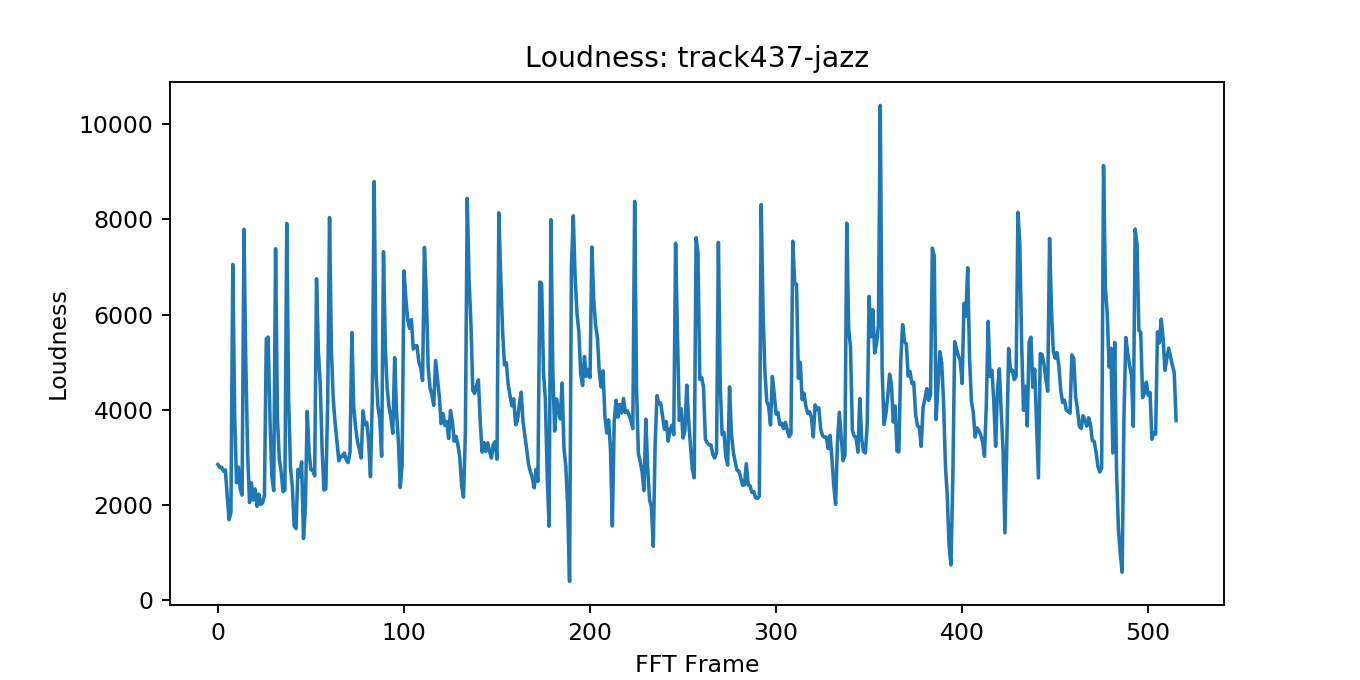
\includegraphics[width=0.9\textwidth]{loudness_track437-jazz}
		\caption{'track437-jazz.wav'}
		\label{fig:loudness_jazz}
	\end{subfigure}
	\begin{subfigure}[t]{\hsize}
		\centering
		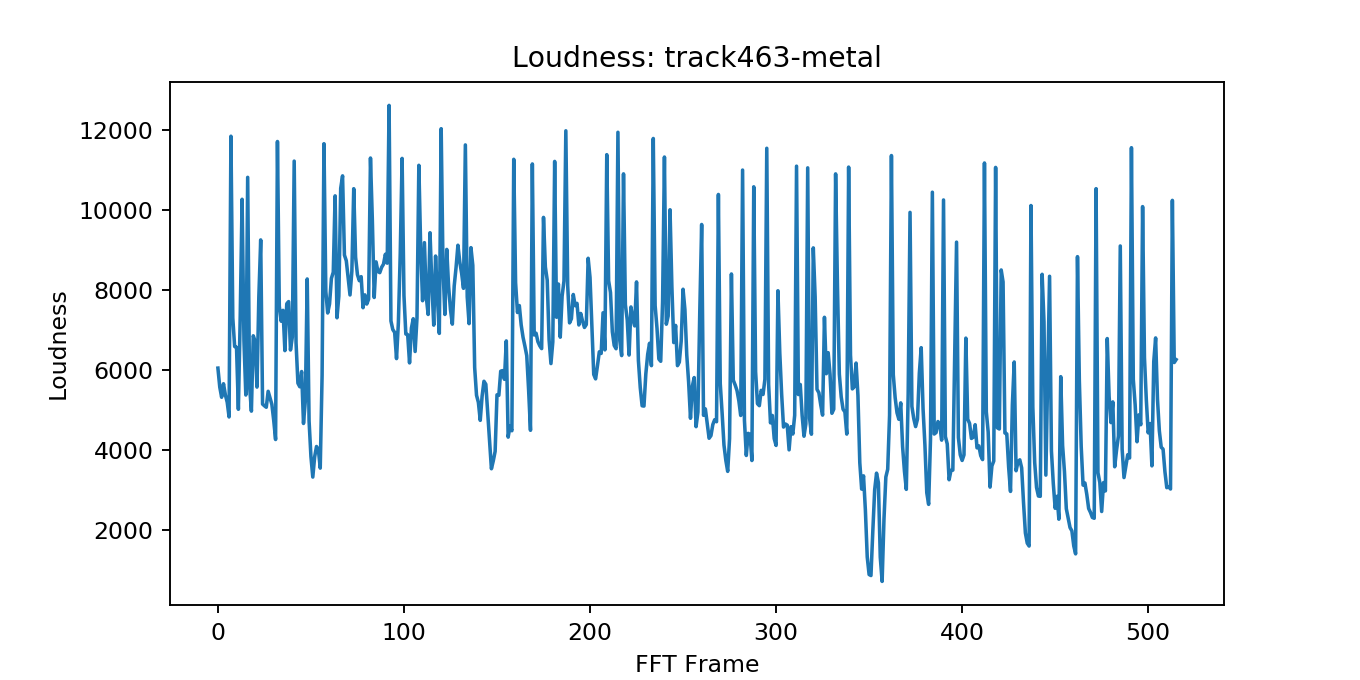
\includegraphics[width=0.9\textwidth]{loudness_track463-metal}
		\caption{'track463-metal.wav'}
		\label{fig:loudness_metal}
	\end{subfigure}
	\caption{Loudness vs. frame}
\end{figure}
\clearpage
\begin{figure}[tb]\ContinuedFloat
	\begin{subfigure}[t]{\hsize}
		\centering
		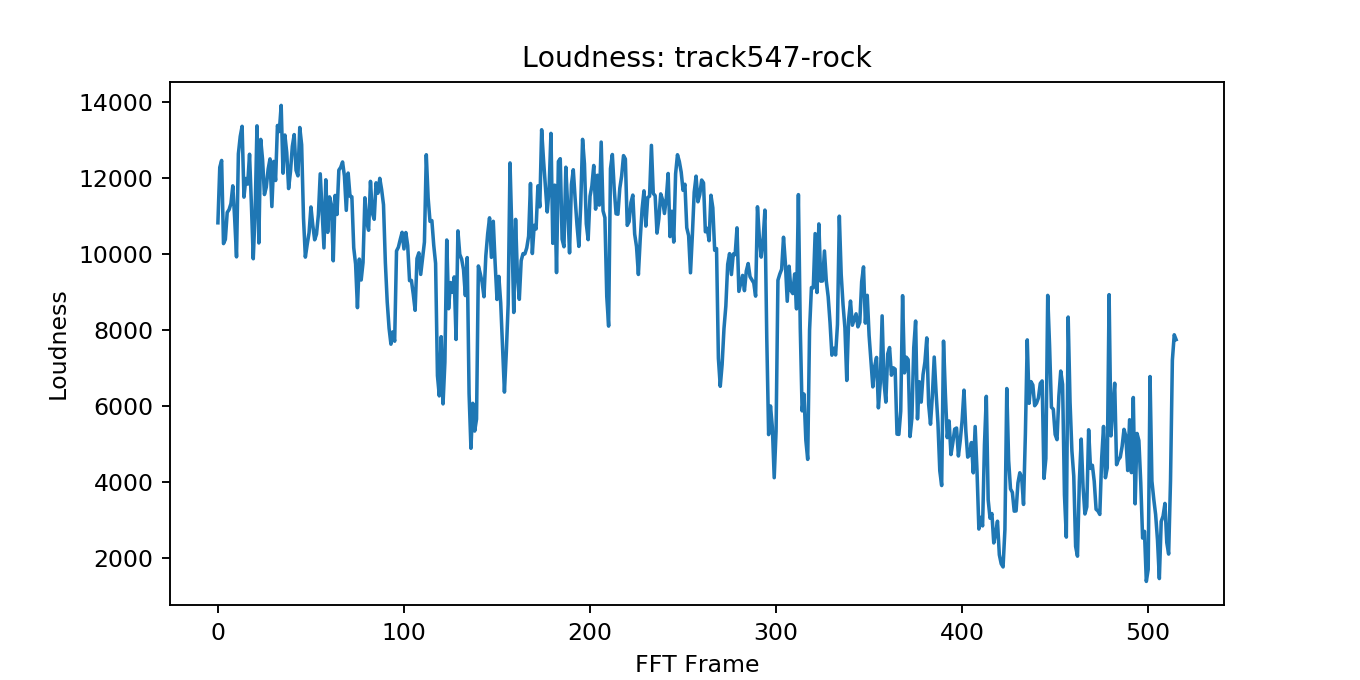
\includegraphics[width=0.9\textwidth]{loudness_track547-rock}
		\label{fig:loudness_rock}
		\caption{'track547-rock.wav'}
	\end{subfigure}
	\begin{subfigure}[t]{\hsize}
		\centering
		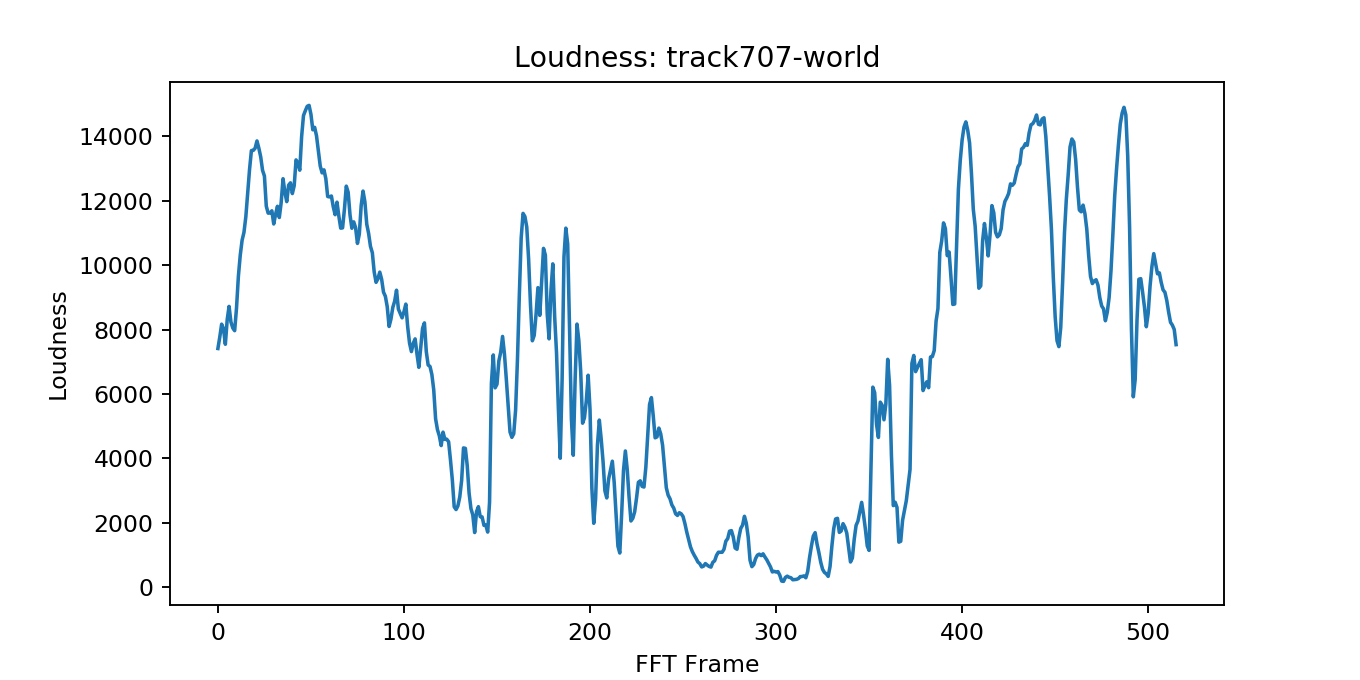
\includegraphics[width=0.9\textwidth]{loudness_track707-world}
		\caption{'track707-world.wav'}
		\label{fig:loudness_world}
	\end{subfigure}
\caption{Loudness vs. frame}
\end{figure}
\clearpage

\paragraph*{Comments} While each of the plots in figure \ref{fig:loudness} has its own characteristics, loudness is not the best tool for characterizing genres. Figure \ref{fig:loudness_electronic} shows the uniformity of the track over time and contrasts with figure \ref{fig:loudness_world} as well as figure \ref{fig:loudness_classical}, however it would be hard to distinguish between figure \ref{fig:loudness_electronic} and figure \ref{fig:loudness_metal}. However, these plots do give a good sense of the progression of each song during the sample considered.

\subsection{Zero Crossing Rate}
\paragraph*{} The zero crossing rate (ZCR) is the average number of times the audio signal crosses the zero amplitude line per unit time. It is related to pitch height and correlated to the noise in the signal. For this lab, ZCR is defined as:

\begin{equation}
ZCR(n)=\frac{1}{N-1}\sum_{m=1}^{N-1}\frac{1}{2}|sgn(x(nN+m))-sgn(x(nN+m-1))|.
\end{equation}

See section \ref{app:zcr} for Python implementation.

\paragraph{Results} Again, we display the output of computed ZCR for one track of each genre in the figures below.

\begin{figure}[tb]
	\centering
	\begin{subfigure}[t]{\hsize}
		\centering
		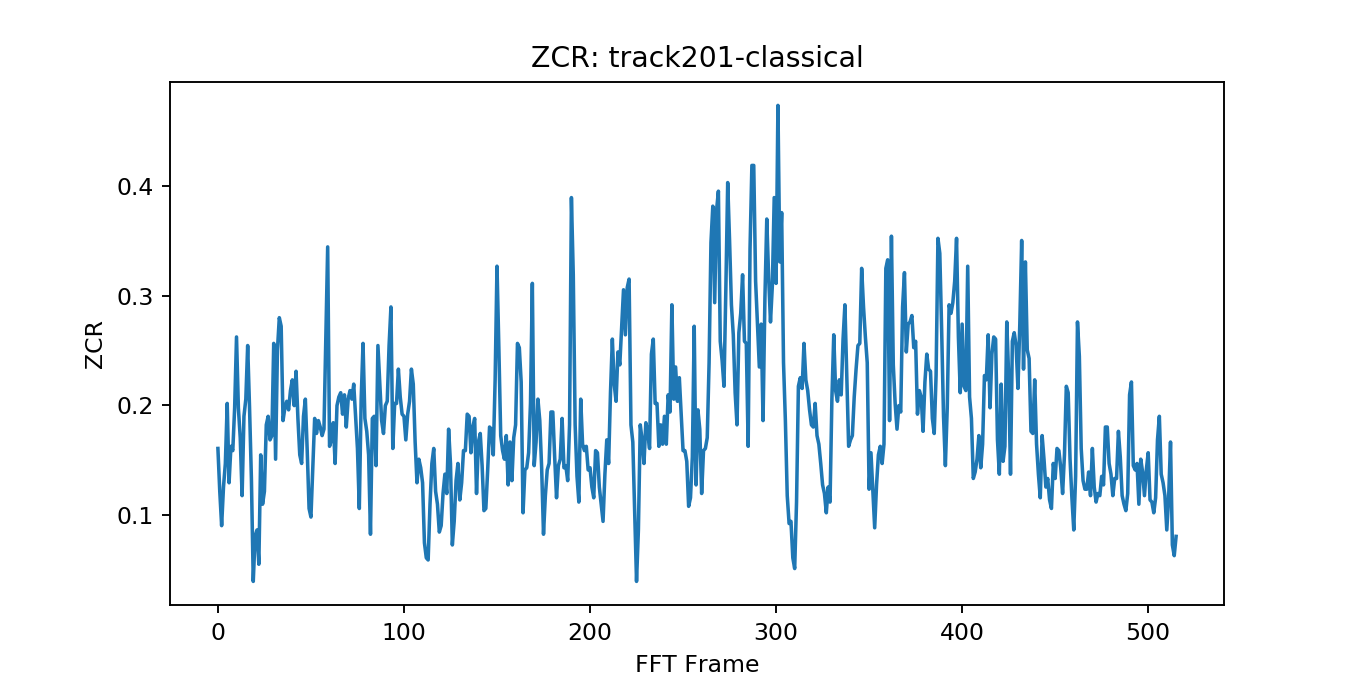
\includegraphics[width=0.9\textwidth]{zcr_track201-classical}
		\caption{'track201-classical.wav'}
		\label{fig:zcr_classical}
	\end{subfigure}
	\begin{subfigure}[t]{\hsize}
		\centering
		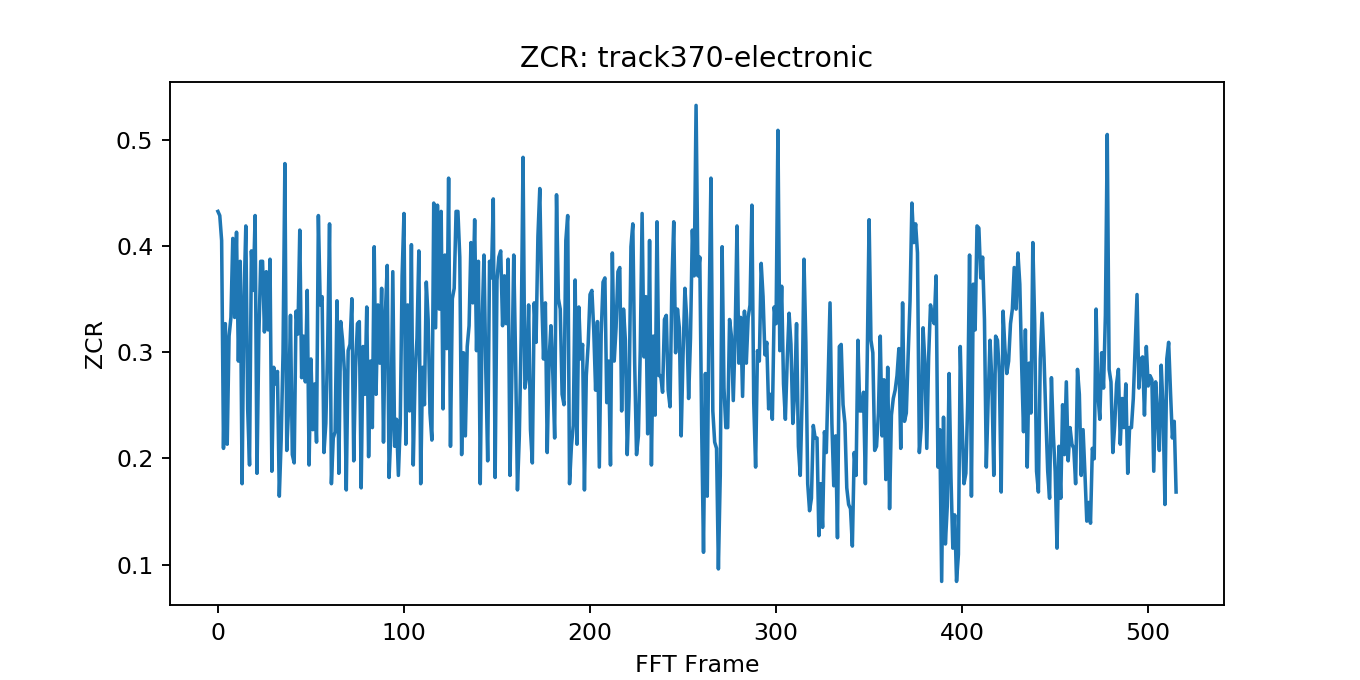
\includegraphics[width=0.9\textwidth]{zcr_track370-electronic}
		\caption{'track370-electronic.wav'}
		\label{fig:zcr_electronic}
	\end{subfigure}
	\caption{ZCR vs. frame \label{fig:zcr}}
\end{figure}
\clearpage
\begin{figure}[tb]\ContinuedFloat
	\begin{subfigure}[t]{\hsize}
		\centering
		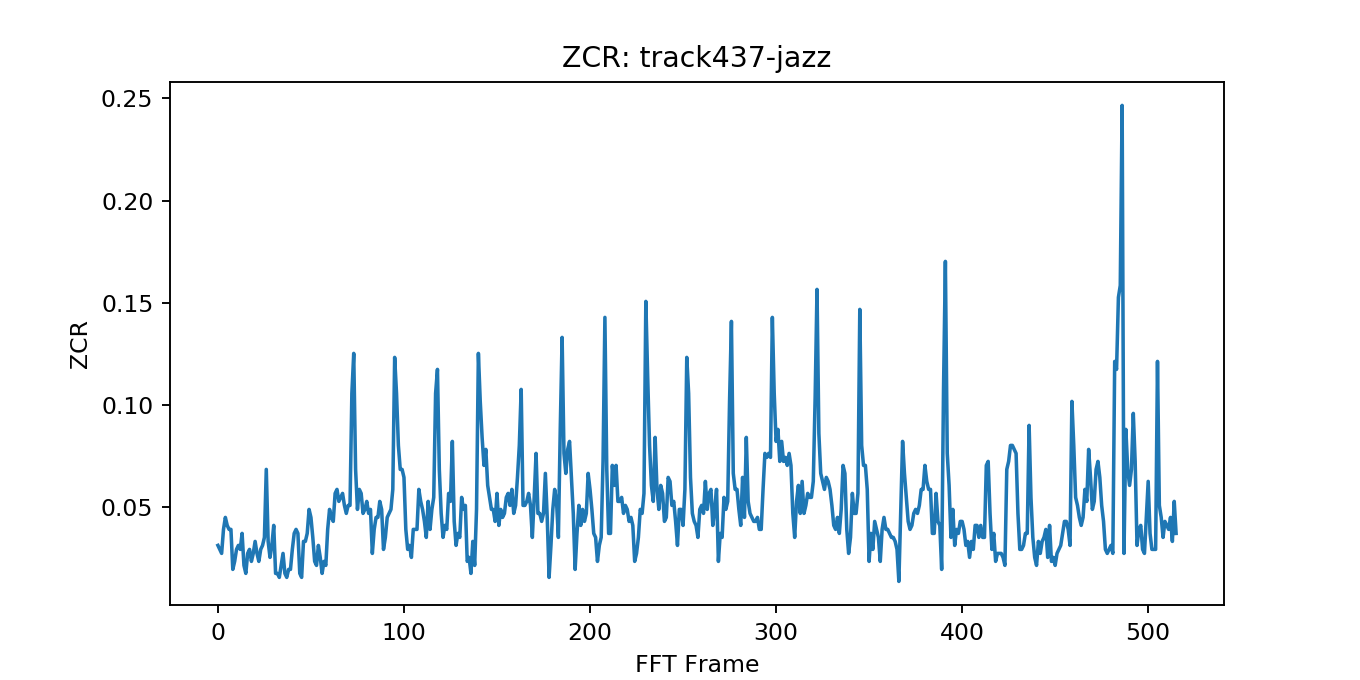
\includegraphics[width=0.9\textwidth]{zcr_track437-jazz}
		\caption{'track437-jazz.wav'}
		\label{fig:zcr_jazz}
	\end{subfigure}
	\begin{subfigure}[t]{\hsize}
		\centering
		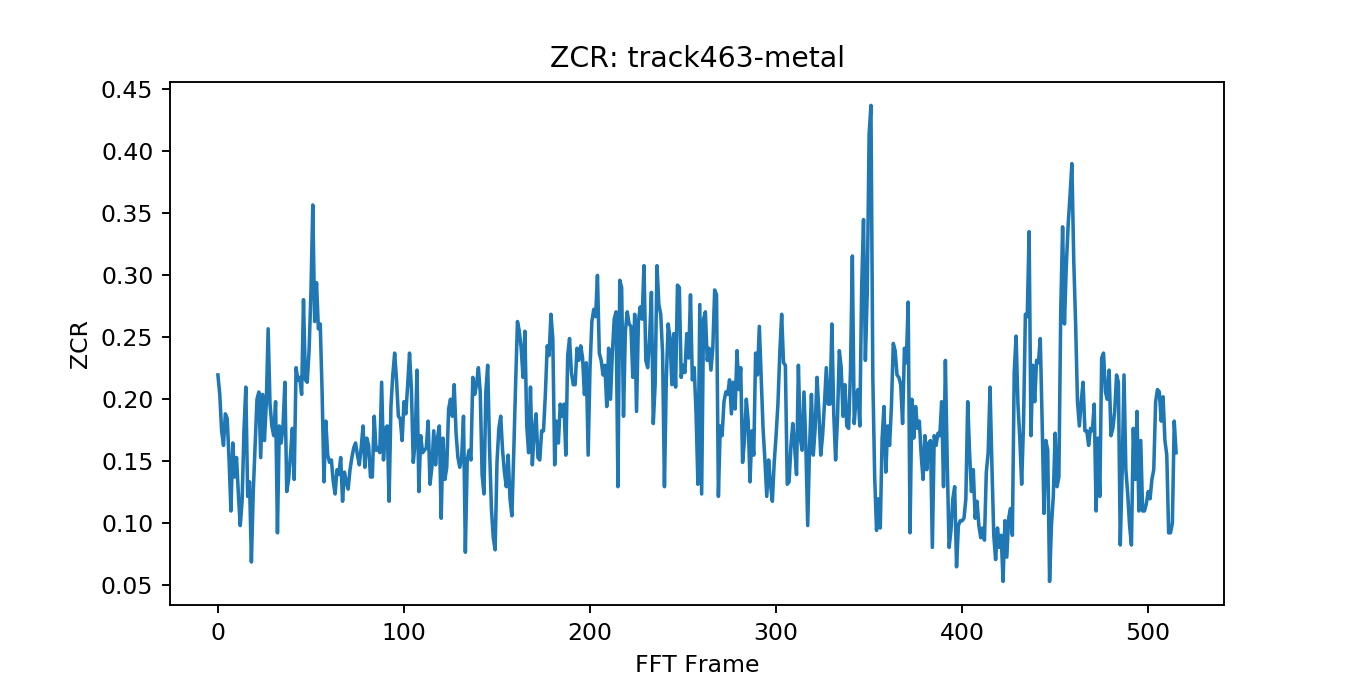
\includegraphics[width=0.9\textwidth]{zcr_track463-metal}
		\caption{'track463-metal.wav'}
		\label{fig:zcr_metal}
	\end{subfigure}
	\caption{ZCR vs. frame}
\end{figure}
\clearpage
\begin{figure}[tb]\ContinuedFloat
	\begin{subfigure}[t]{\hsize}
		\centering
		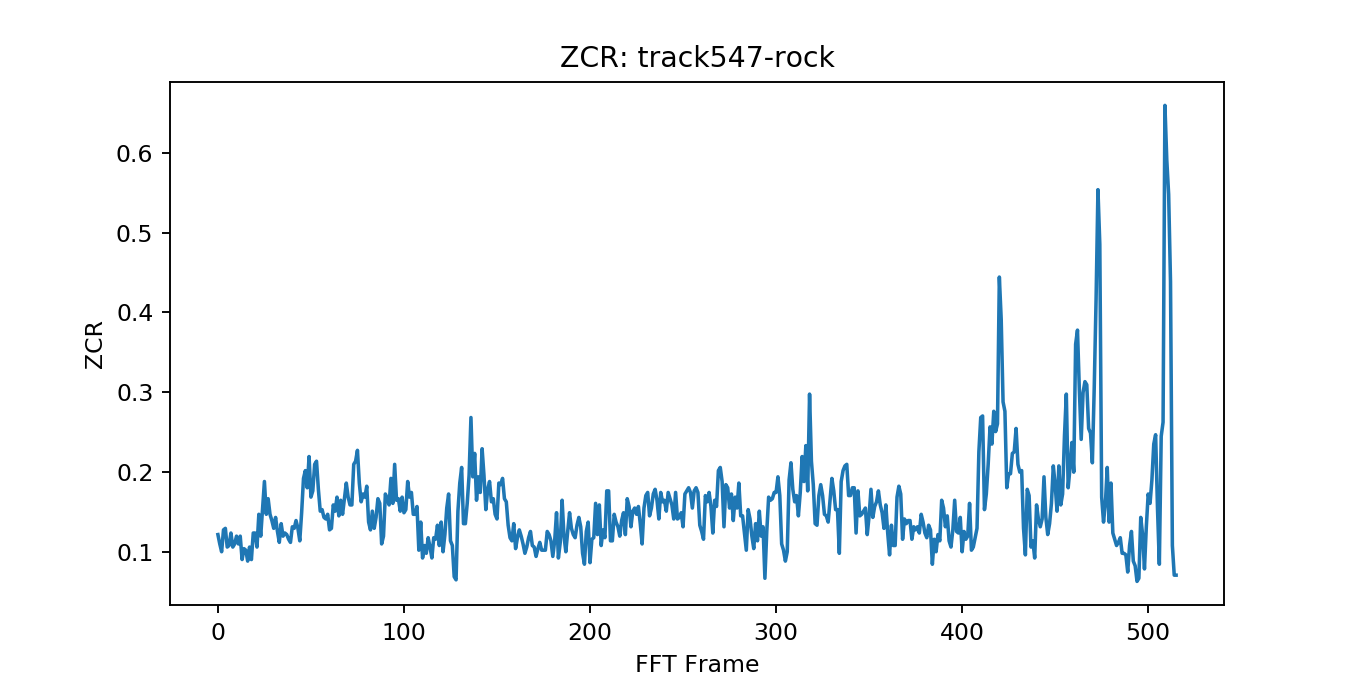
\includegraphics[width=0.9\textwidth]{zcr_track547-rock}
		\caption{'track547-rock.wav'}
		\label{fig:zcr_rock}
	\end{subfigure}
	\begin{subfigure}[t]{\hsize}
		\centering
		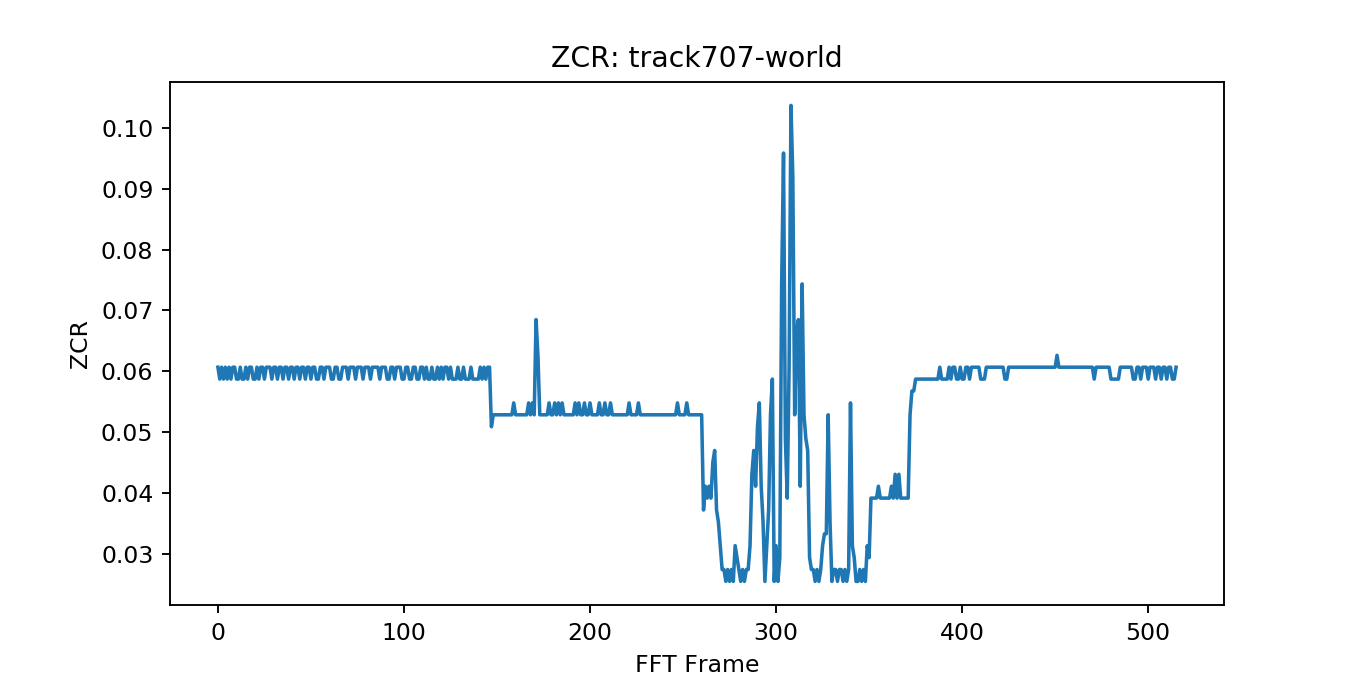
\includegraphics[width=0.9\textwidth]{zcr_track707-world}
		\caption{'track707-world.wav'}
		\label{fig:zcr_world}
	\end{subfigure}
	\caption{ZCR vs. frame}
\end{figure}

\paragraph{Comments} From the plots in figure \ref{fig:zcr} we can definitely see some variability between genres. For example, the world track in \ref{fig:zcr_world} is easily distinguishable, however most of the other tracks are similar enough that this is also not likely a good measurement for classifying genre. This can be supported by the similarity between jazz (\ref{fig:zcr_jazz}) and rock (\ref{fig:zcr_rock}).

\pagebreak

\section{Spectral (Frequency) Analysis}
\paragraph*{} Sound, by nature is made up of many different frequencies or notes of different pitch. Thus it is natural to analyze audio in the spectral (frequency) domain. 
\paragraph{Method} As discussed in the introduction, we will accomplish our spectral analysis using a STFT, which decomposes short-time frames of a signal into discrete frequency bins, maintaining some time-domain relevance within the spectral domain. Then, we will perform some statistical analysis on the signal in an attempt to characterize some songs.
\paragraph*{} Rather than directly splitting each of our $N=512$ frames, we will convolve (a fancy term for multiplication in the frequency domain) a taper window, $w$, with the signal and take the Fourier transform (FT). Since the signal is real, and we are concerned only with the magnitude, we will compute the FT of only half of the frequency spectrum to arrive at $N/2=256$ frequency bins for each of our $N=512$ frames. Finally, for the purposes of this analysis, we are interested in the power spectrum of the original song, so we take the magnitude squared (i.e. $|X_n(k)|^2$, as a function of the frame index $n$ and frequency index $k$). See section \ref{app:frequencydomain} for Python implementation.
\paragraph{DTFT Window Derivation} To give some motivation for the taper window, $w$, we will derive the theoretical discrete-time Fourier transform (DTFT) for a given signal $x[n]$ where,

\begin{align} \label{eqn:rect}
x[n] &= 1, && -N/2 \leq n \leq N/2 \\
x[n] &= 0, && \text{else}
\end{align}

Recall the definition of the DTFT.

\begin{equation} \label{eqn:dtft}
X(\omega)=\sum_{n=-\infty}^{\infty} x[n]e^{-j\omega n}.
\end{equation}

Since $x[n]\neq 0$ over only a subset of values in the DTFT range, equation \eqref{eqn:dtft} becomes,

\begin{align}
X(\omega) &= \sum_{n=-N/2}^{N/2} x[n]e^{-j\omega n}  \nonumber \\
		  &= \sum_{n=-N/2}^{N/2} \left(e^{-j\omega}\right)^n &\text{which we can rewrite as} &\text{(a geometric series)} \nonumber \\
		  &= e^{j\omega N/2} \frac{1-\left(e^{-j\omega}\right)^{N+1}}{1-e^{-j\omega}} &\text{factoring,} \nonumber \\
		  &= e^{j\omega N/2} \frac{e^{-j\omega (N+1)/2} \left( e^{j\omega (N+1)/2} - e^{-j\omega (N+1)/2} \right)}{e^{-j\omega/2} \left( e^{j\omega/2} - e^{-j\omega/2} \right)} \nonumber \\
		  &= \frac{e^{j\omega (N+1)/2} - e^{-j\omega (N+1)/2}}{e^{j\omega/2} - e^{-j\omega/2}} &\text{and by Euler's formula,} \nonumber \\
X(\omega) &= \frac{sin(\frac{\omega(N+1)}{2})}{sin(\frac{\omega}{2})} \label{eqn:sinc}
\end{align}

\pagebreak

\begin{figure}
	\centering
	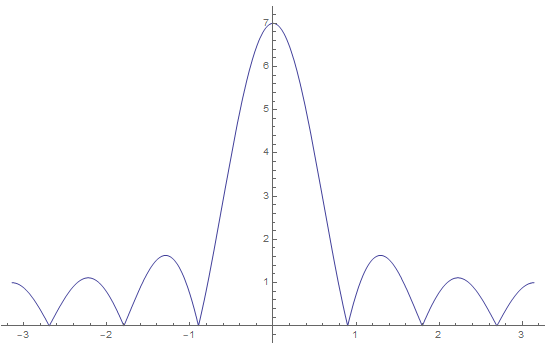
\includegraphics[width=0.9\textwidth]{sinc}
	\caption{Plot of \eqref{eqn:sinc} with $\omega=[-\pi,\pi]$ ($N=6$).}
	\label{fig:sinc}
\end{figure}

Equation \eqref{eqn:sinc}, the magnitude of which is plotted in figure \ref{fig:sinc}, is easily recognized as the $sinc$ function. Notice the relatively large amplitude side-lobes. If we consider constant total energy of this function when used as a window, the narrow main-lobe will extract each frequency very selectively, with the side-lobes producing frequency leakage. In contrast, if we aim to extract frequencies with minimal leakage, we could choose a window with a wider main-lobe. In that case, the energy would be more concentrated at the central frequency, albeit less selectively. In this lab, we will focus on some windows that are relatively good approximations to a $sinc$ window, but with no side-lobes, so the frequency leakage is essentially eliminated. The tradeoff is that we produce a low-passed version of the original signal at the output of the window operation. 

\paragraph{Windowing a Signal} The process of multiplying a signal $x[n]$ by a window $w[n]$ is relatively straightforward. We consider the operation in the time-domain and derive the frequency-domain equivalence.

\begin{equation} \label{eqn:wintime}
y[n] = x[n]w[n]
\end{equation}

Recall that multiplication in time is a convolution in frequency, such that 
\begin{align}
Y(\omega) 	&= X(\omega)*W(\omega) \nonumber \\
			&= \sum_{k=-\infty}^{+\infty} W(\omega)X(\omega-k) \label{eqn:conv} \\
			&= \sum_{k=-\pi}^{\pi} \frac{sin(\frac{\omega(N+1)}{2})}{sin(\frac{\omega}{2})}X(\omega-k) \label{eqn:windowed}
\end{align}

where \eqref{eqn:conv} is the definition of convolution\cite{convolution} and \eqref{eqn:windowed} is the output of the window operation in frequency. We will use this over a sequence of 'frames' of a DTFT algorithm in Python to generate a spectrogram of a signal.

\pagebreak

\subsection{Spectrogram} As promised, we will be implementing a STFT. In Python, we will use the \verb|scipy.signal.spectrogram| function to automate this. However, we first need a window. For this, we will use the library function, \verb|scipy.signal.get_window| which allows us to quickly generate taper windows of the same size as our STFT frames. There are many choices of windows, but we will look at the 'Hann' and 'Blackman' windows. See figure \ref{fig:windows}.

\begin{figure}[ht]
	\centering
	\begin{subfigure}[t]{\hsize}
	\centering
		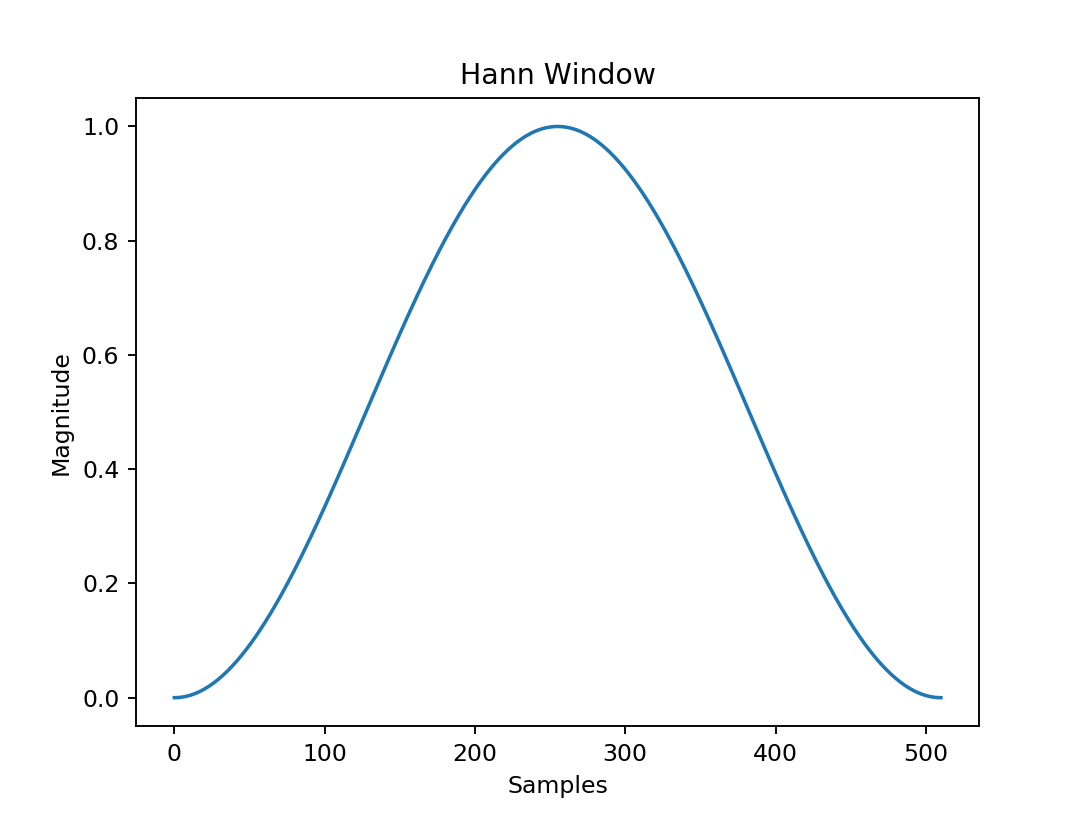
\includegraphics[width=0.6\textwidth]{hann}
		\caption{Hann window}
		\label{fig:hann}
	\end{subfigure}
	\begin{subfigure}[t]{\hsize}
		\centering
		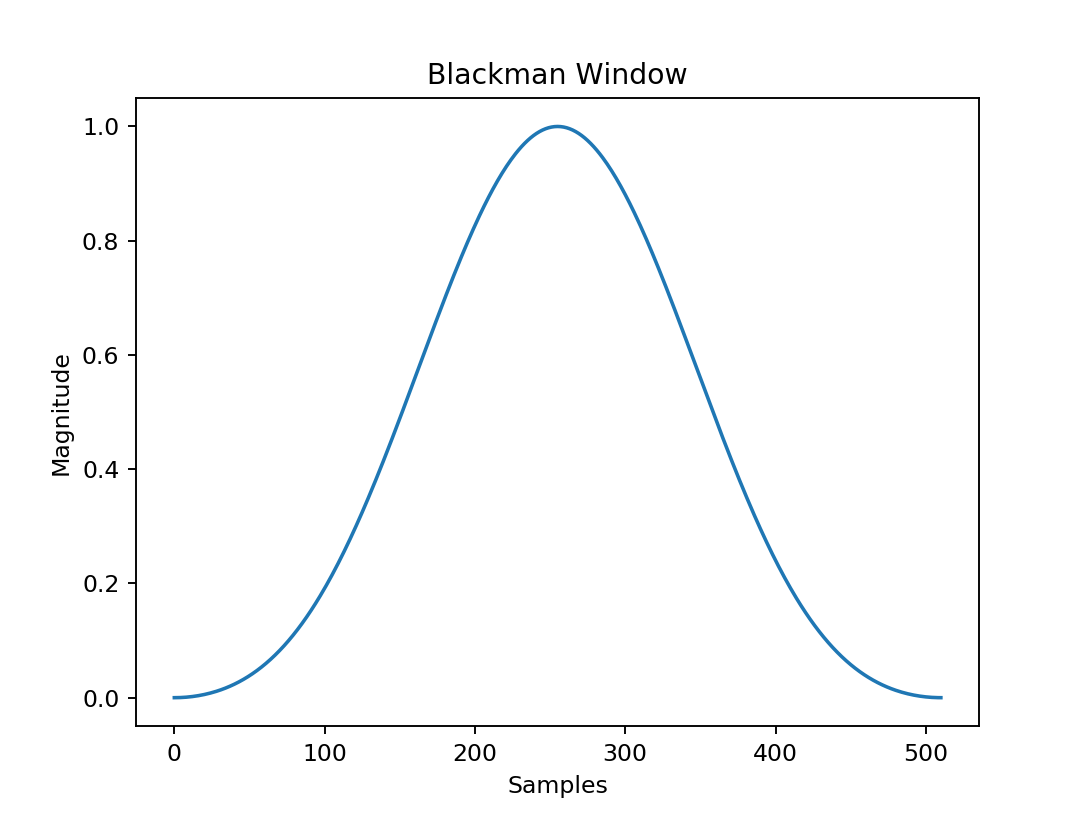
\includegraphics[width=0.6\textwidth]{blackman}
		\caption{Blackman window}
		\label{fig:blackman}
	\end{subfigure}
	\caption{Windows}
	\label{fig:windows}
\end{figure}

\paragraph*{} As you can see, the Hann window (\ref{fig:hann}) tapers a little less steeply than the Blackman window (\ref{fig:blackman}).
\clearpage

\begin{figure}[tb]
	\centering
	\begin{subfigure}[t]{\hsize}
		\centering
		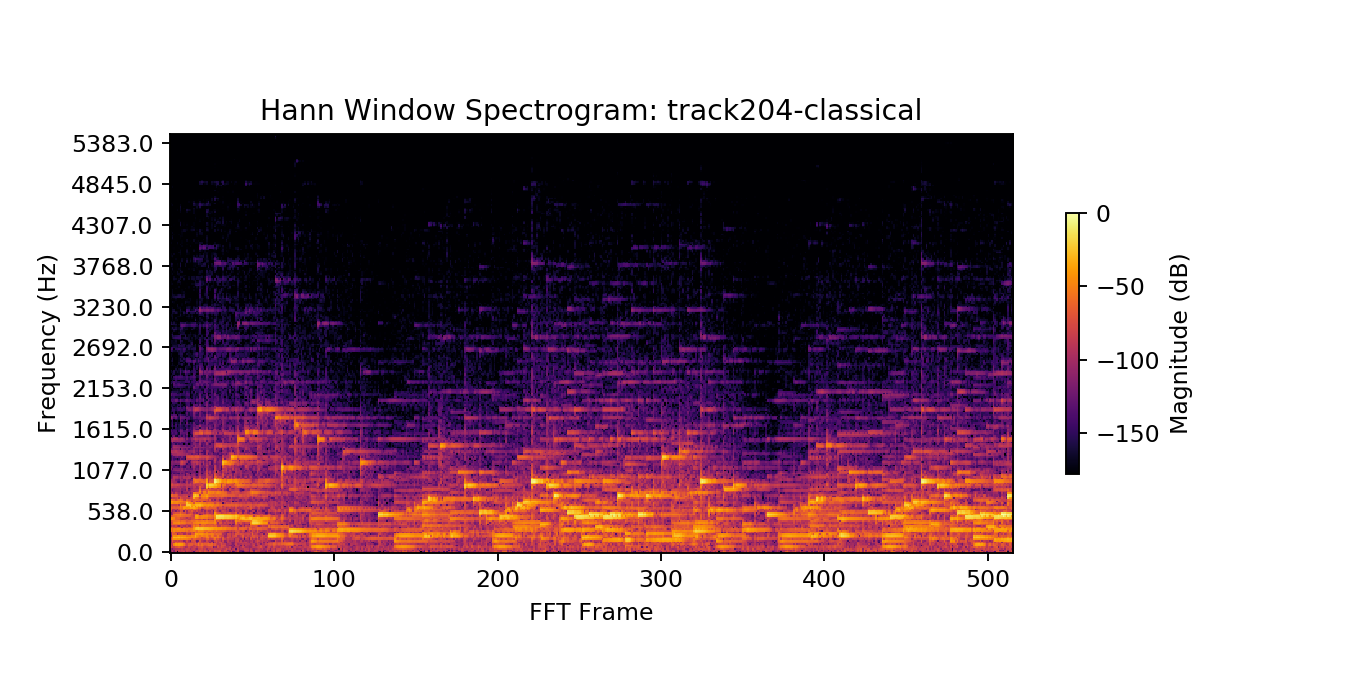
\includegraphics[width=0.9\textwidth]{powerHann_track204-classical}
		\caption{Spectrogram of 'track204-classical' using a Hann window}
		\label{fig:hann_classical}
	\end{subfigure}
	\begin{subfigure}[t]{\hsize}
		\centering
		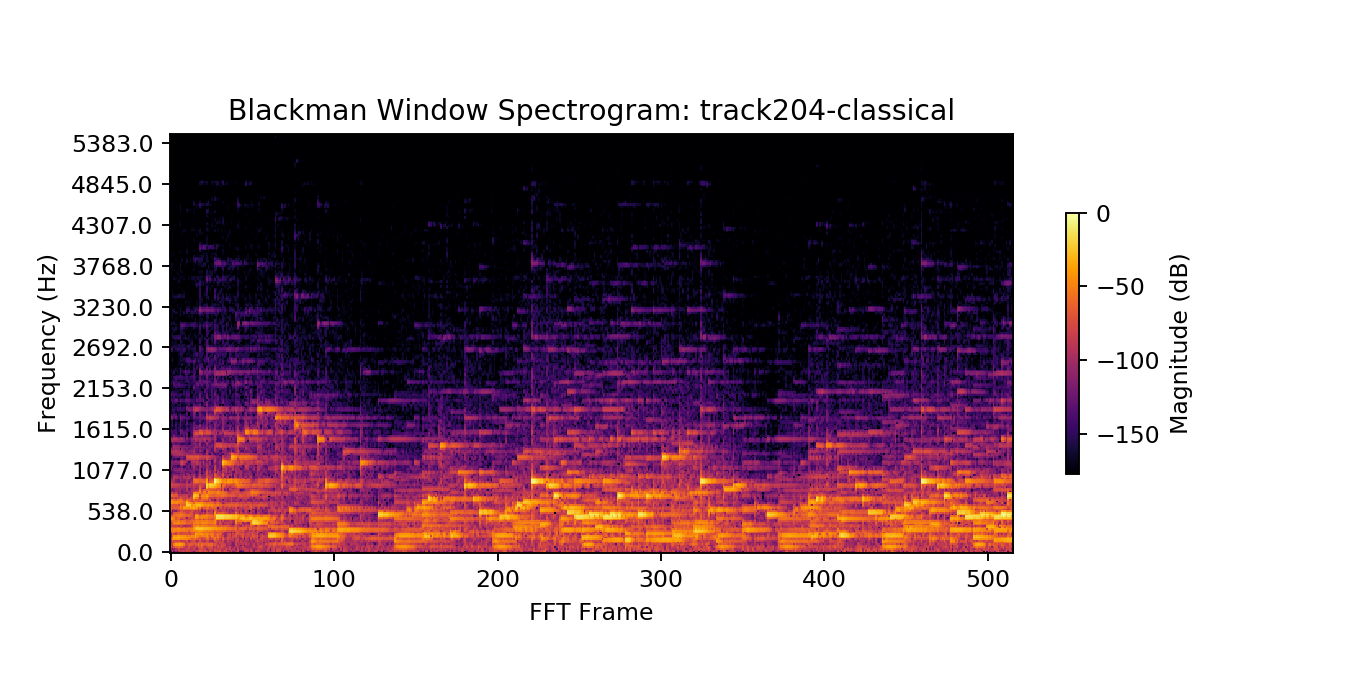
\includegraphics[width=0.9\textwidth]{powerBlack_track204-classical}
		\caption{Spectrogram of 'track204-classical' using a Blackman window}
		\label{fig:black_classical}
	\end{subfigure}
	\caption{Hann vs. Blackman windows for a classical music track}
	\label{fig:windows_classical}
\end{figure}
\clearpage

\begin{figure}[tb]
	\centering
	\begin{subfigure}[t]{\hsize}
		\centering
		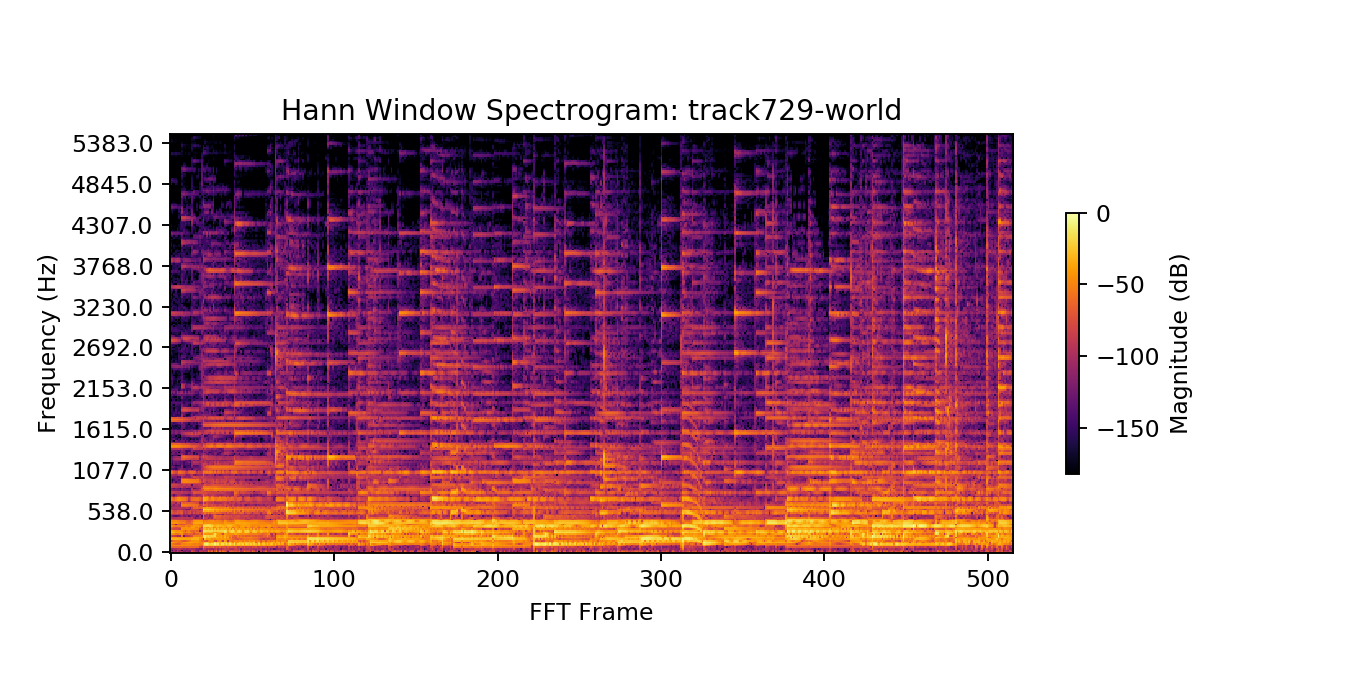
\includegraphics[width=0.9\textwidth]{powerHann_track729-world}
		\caption{Spectrogram of 'track729-world' using a Hann window}
		\label{fig:hann_world}
	\end{subfigure}
	\begin{subfigure}[t]{\hsize}
		\centering
		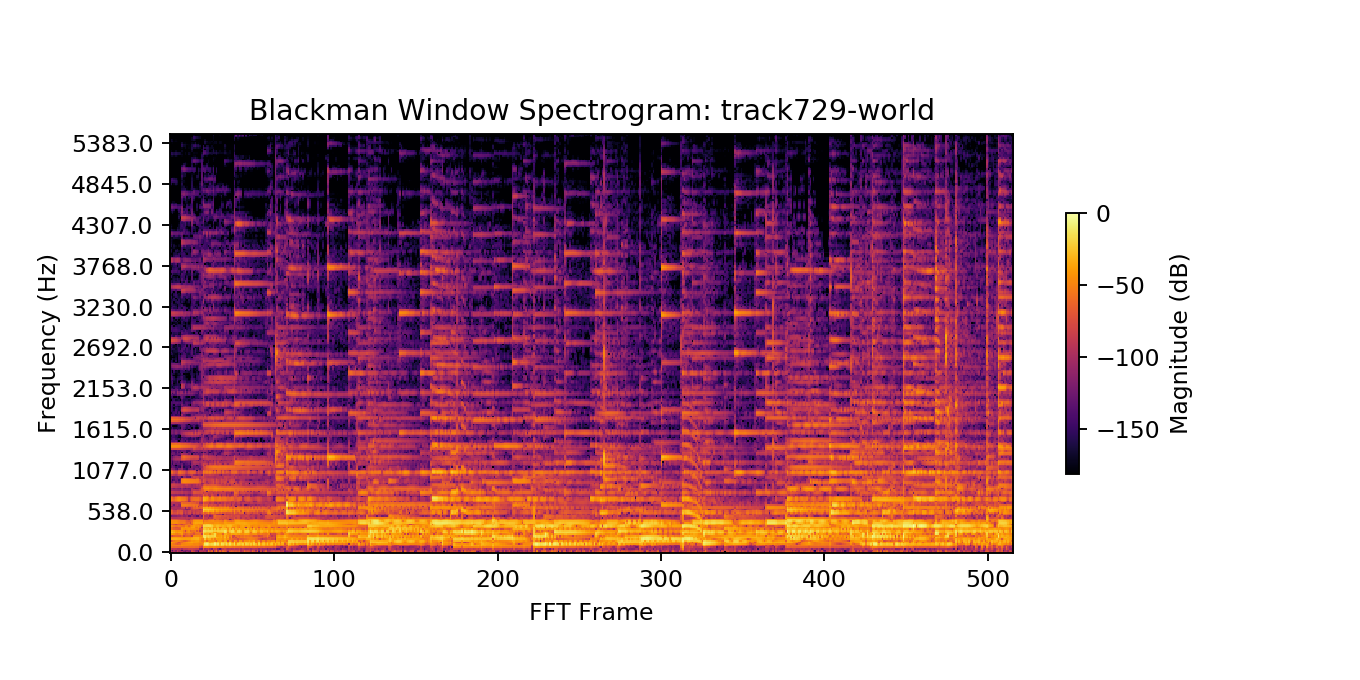
\includegraphics[width=0.9\textwidth]{powerBlack_track729-world}
		\caption{Spectrogram of 'track729-world' using a Blackman window}
		\label{fig:black_world}
	\end{subfigure}
	\caption{Hann vs. Blackman windows for a classical music track}
	\label{fig:windows_world}
\end{figure}

See section \ref{app:spectrogram} for implementation in Python.

\paragraph{Comments} If you look closely at figures \ref{fig:hannCrop} and \ref{fig:blackmanCrop}, you can see that there is more spectral bleeding in the Blackman window, however the magnitude of center frequencies is relatively higher. We will proceed with analysis using only the Blackman window.

\begin{figure}[ht]
	\centering
	\begin{subfigure}[h]{0.45\textwidth}
		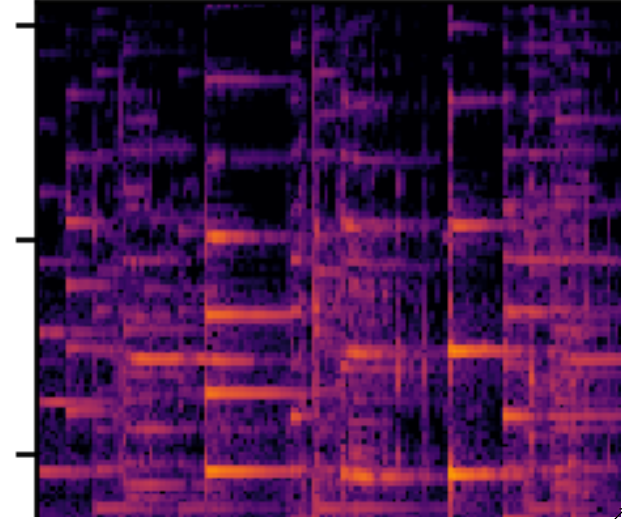
\includegraphics[width=\textwidth]{hannCrop}
		\caption{Hann Window}
		\label{fig:hannCrop}
	\end{subfigure}
	\begin{subfigure}[h]{0.45\textwidth}
		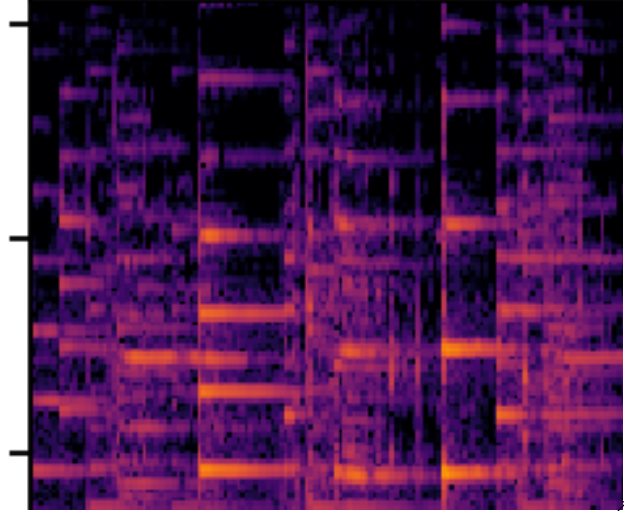
\includegraphics[width=\textwidth]{blackmanCrop}
		\caption{Blackman Window}
		\label{fig:blackmanCrop}
	\end{subfigure}
	\caption{A closer look at Hann and Blackman windows.}
	\label{fig:windowCloseup}
\end{figure}

\pagebreak

\subsection{Spectral Centroid and Spread}
\paragraph*{} We wish to find the 'center of mass' of each frame in a spectrogram and will call this the spectral centroid. The centroid can be used to quantify sound sharpness or brightness. Additionally, we would like to find the spectral spread, or width of the spectrum around the centroid. Thus, we can then compare tone-like and noise-like sounds. For these concepts, we will treat the normalized magnitude of a spectral coefficient as if it were a 'probability' of that particular frequency. Then, for frame $n$, we have the 'probability' of frequency $k$

\begin{equation} \label{eqn:P}
P_n(k) = \frac{|X_n(k)|}{\sum_{l=0}^{K} |X_n(l)|}
\end{equation}

Which we can then use to define the spectral centroid as

\begin{equation}
\mu_n = \sum_{k=0}^{K} kP_n(k)
\end{equation}

And the spectral spread for frame $n$ is the standard deviation given by

\begin{equation}
\sigma_n = \sqrt{\sum_{k=0}^{K} [k-\mu_n]^2 P_n(k)}
\end{equation}

The spectral centroid and spread were calculated for a classical, jazz, and metal song and a time-domain plot is shown in figure \ref{fig:cs}. See section \ref{app:centroidspread} for Python implementation.

\pagebreak

\begin{figure}[tb]
	\centering
	\begin{subfigure}[t]{\hsize}
		\centering
		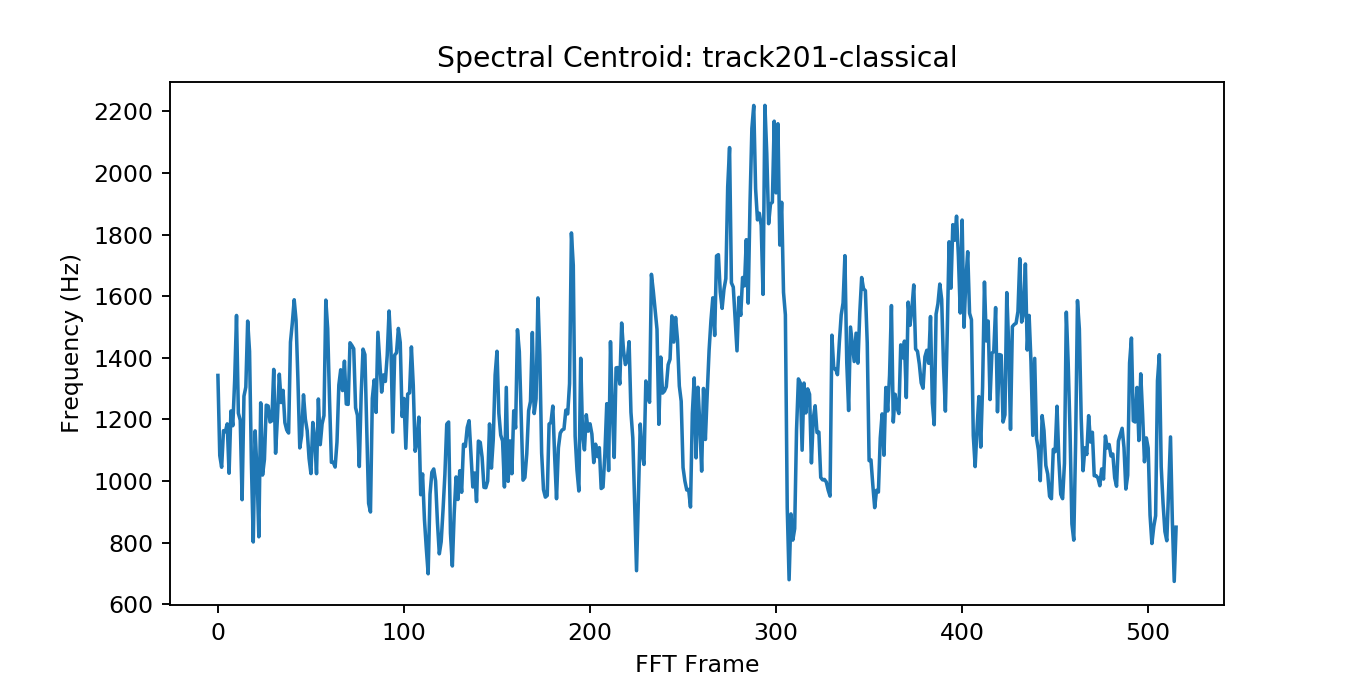
\includegraphics[width=0.9\textwidth]{centroid_track201-classical}
		\caption{Spectral centroid of 'track201-classical' as a function of frame number.}
		\label{fig:centroid_classical}
	\end{subfigure}
	\begin{subfigure}[t]{\hsize}
		\centering
		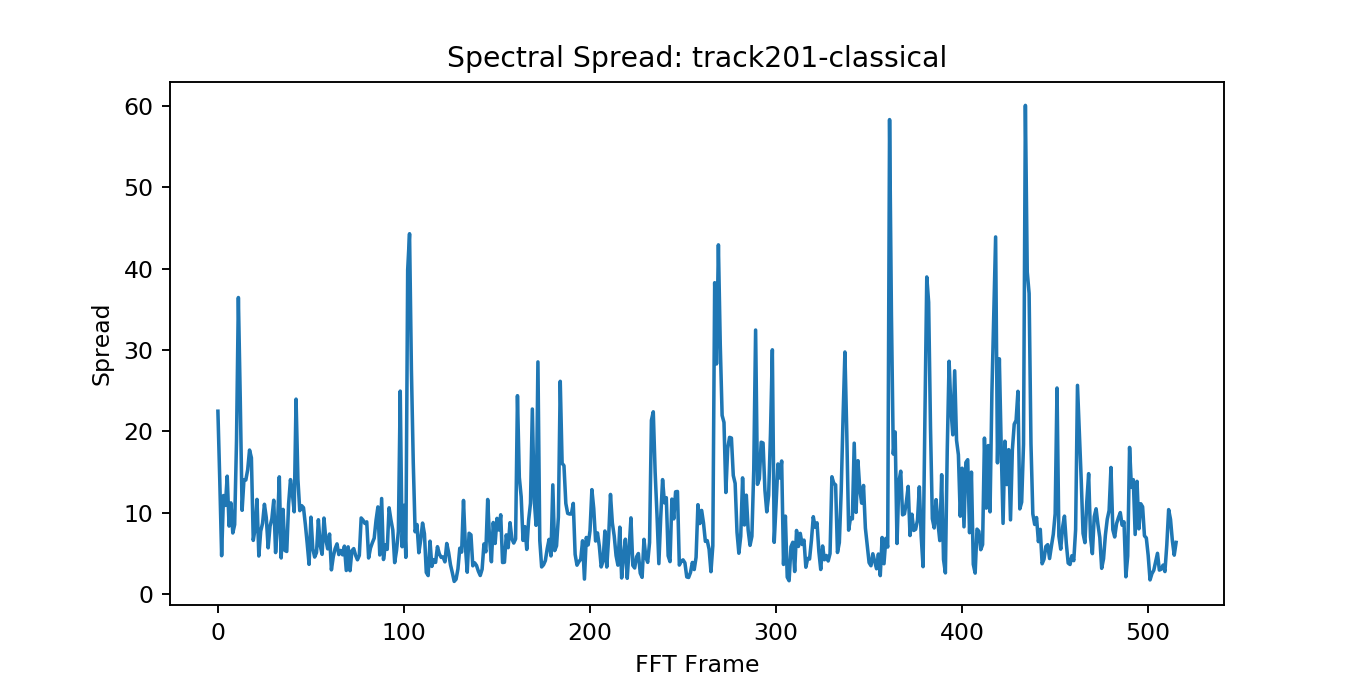
\includegraphics[width=0.9\textwidth]{spread_track201-classical}
		\caption{Spectral spread of 'track201-classical' as a function of frame number.}
		\label{fig:spread_classical}
	\end{subfigure}
	\caption{Centroid and spread \label{fig:cs}}
\end{figure}
\clearpage

\begin{figure}[tb]\ContinuedFloat
	\begin{subfigure}[t]{\hsize}
		\centering
		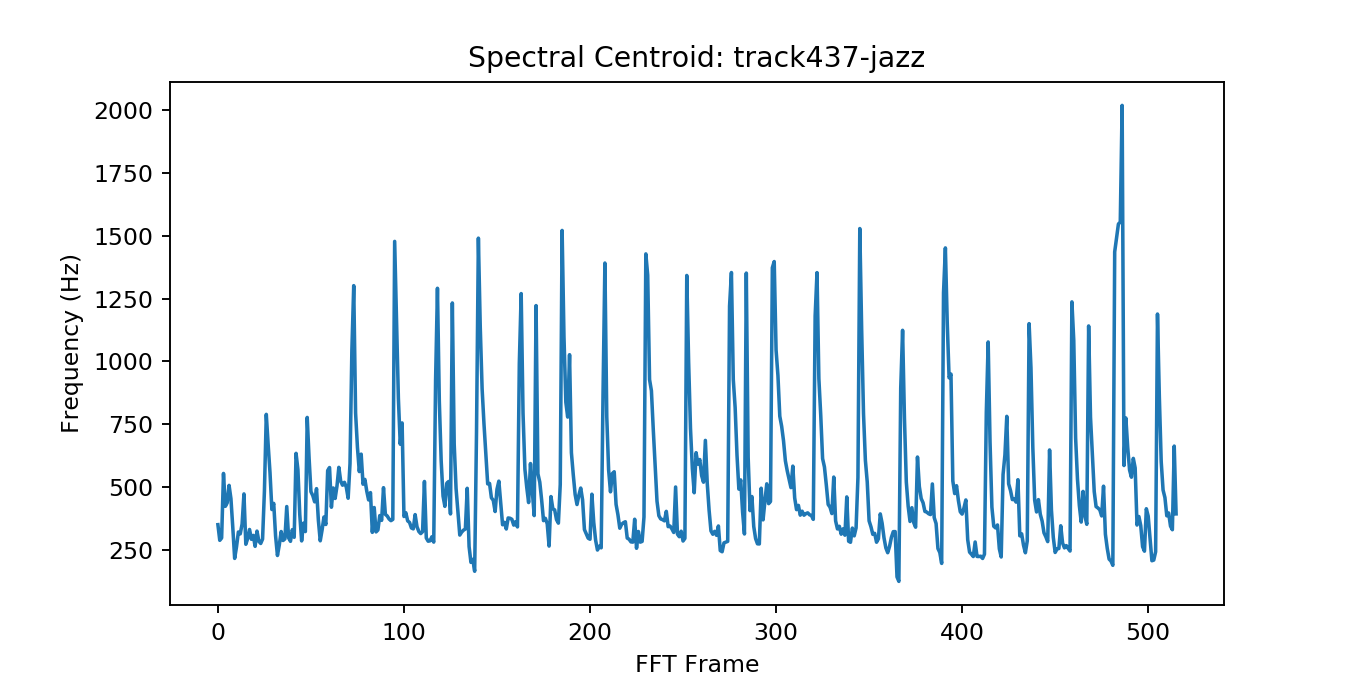
\includegraphics[width=0.9\textwidth]{centroid_track437-jazz}
		\caption{Spectral centroid of 'track437-jazz' as a function of frame number.}
		\label{fig:centroid_jazz}
	\end{subfigure}
	\begin{subfigure}[t]{\hsize}
		\centering
		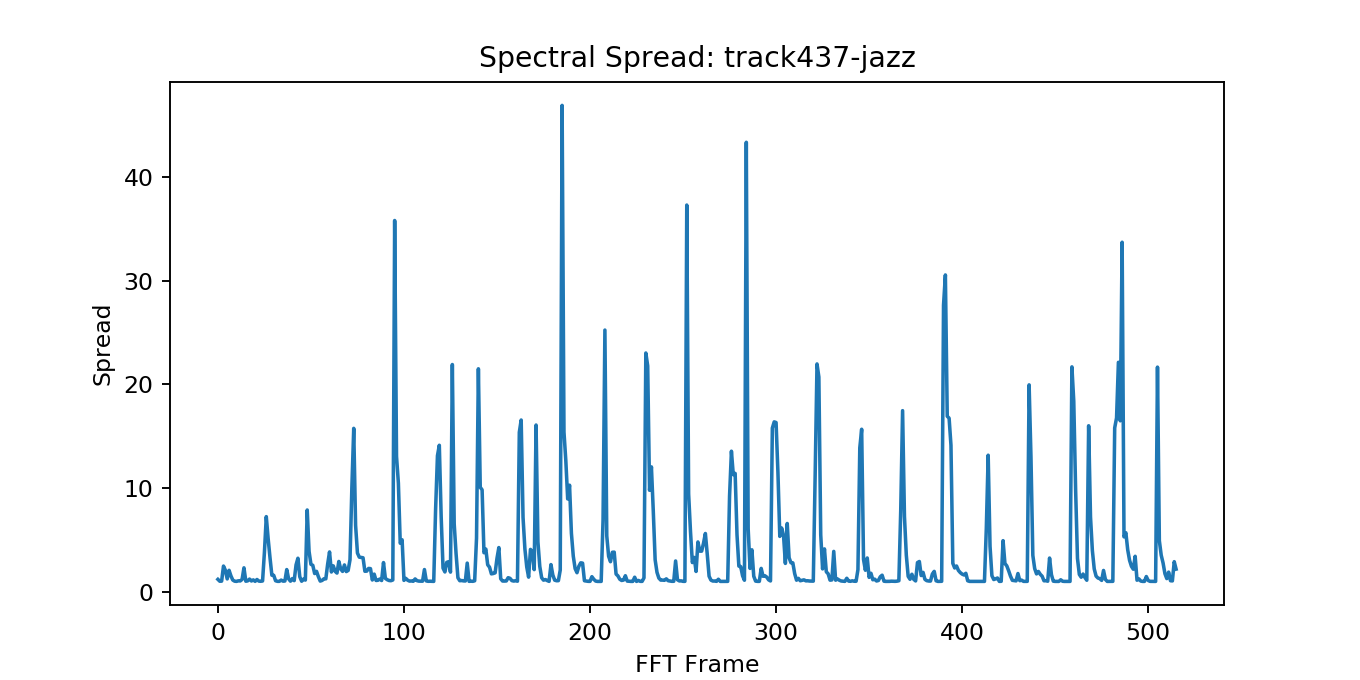
\includegraphics[width=0.9\textwidth]{spread_track437-jazz}
		\caption{Spectral spread of 'track437-jazz' as a function of frame number.}
		\label{fig:spread_jazz}
	\end{subfigure}
	\caption{Centroid and spread}
\end{figure}
\clearpage

\begin{figure}[tb]\ContinuedFloat
	\begin{subfigure}[t]{\hsize}
		\centering
		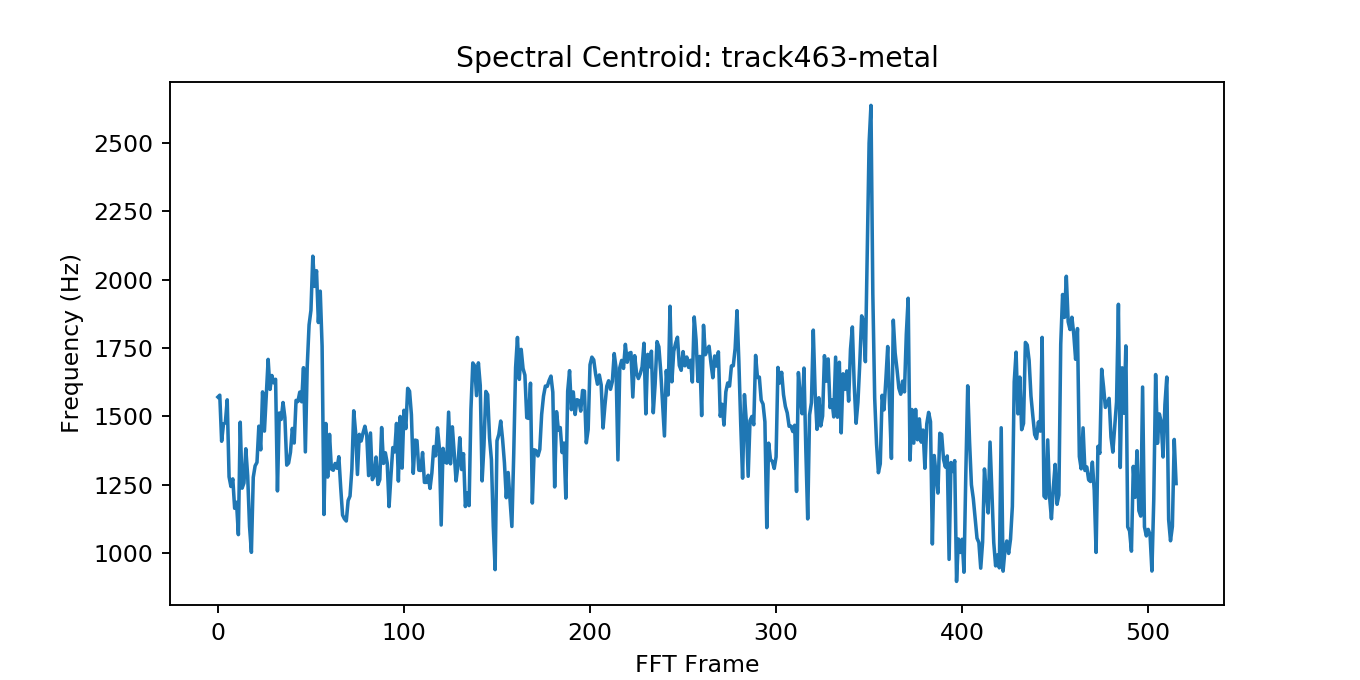
\includegraphics[width=0.9\textwidth]{centroid_track463-metal}
		\caption{Spectral centroid of 'track463-metal' as a function of frame number.}
		\label{fig:centroid_metal}
	\end{subfigure}
	\begin{subfigure}[t]{\hsize}
		\centering
		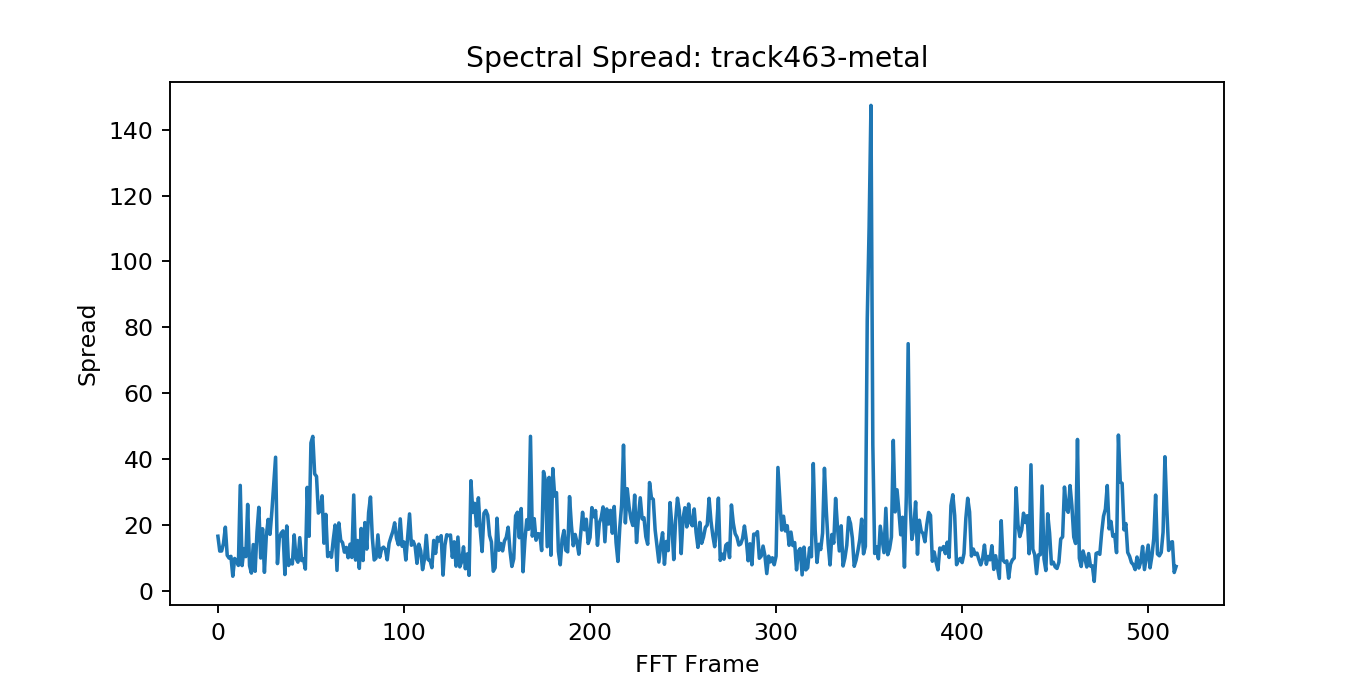
\includegraphics[width=0.9\textwidth]{spread_track463-metal}
		\caption{Spectral spread of 'track463-metal' as a function of frame number.}
		\label{fig:spread_metal}
	\end{subfigure}
	\caption{Centroid and spread}
\end{figure}
\clearpage

\paragraph{Comments} The centroids of this classical track, shown in figure \ref{fig:centroid_classical} the most statistically significant frequency changes from frame to frame, sometimes drastically. This is most likely due to the violin's sharp transitions between tones. Then in the spread (figure \ref{fig:spread_classical}), we can see that there is relatively high spread for many frames, indicating the high tones in the song and their inherent noise (potentially from under-sampling).
\paragraph*{} Then, we see in the analysis of a jazz song (figures \ref{fig:centroid_jazz} and \ref{fig:spread_jazz}) There is a contrast between the percussion and electric keyboard, which is apparent in the consistently alternating peaks and valleys. The spread shows that many of the peaks are also high-frequency and noisy.
\paragraph*{} In the metal track, we see a relatively uniform centroid (figure \ref{fig:centroid_metal}) and spread (figure \ref{fig:spread_metal}) across frames. Notice also the different scales on the vertical axis of these plots, indicating that the metal track is fairly noisy compared to the other two songs, although it appears to have smaller magnitude on first glance. We see a large spike around frame 350 corresponding to a high-pitch yell from the vocalist. In the centroid plot, this can be seen as a spike in frequency with an associated spread due to the timbre of his voice and noise in the signal.
\paragraph*{} Comparing these between genres, notice that the classical and jazz have some similarities, which would make sense based on the similarity of genres, however we can see a contrast in the centroids, due to the electronic composition of the jazz track as opposed to the natural, dissonant composition of the classical. Furthermore, the small spread shown in figure \ref{fig:spread_jazz} indicates that notes were generated electronically. The metal track stands out in a couple regards. Figure \ref{fig:centroid_metal} is vastly different and shows the dense composition in the track, with the centroid in each frame nearing the middle of the frequency spectrum and indicating that the range of frequencies is large at any given point in the song.

\subsection{Spectral Flatness}
\paragraph*{} Spectral flatness is the ratio between the geometric and arithmetic means of the magnitude of the Fourier transform,

\begin{equation}
SF(n) = \frac{\left( \prod_{k=0}^{K} |X_n(k)|\right)^{1/K}}{\frac{1}{K}\sum_{k=0}^{K} |X_n(k)|}
\end{equation}

A very small flatness corresponds to the presence of tonal components while a flatness equal to one corresponds to a very noisy signal. Thus, flatness is a measure of the noisiness of the spectrum.
\paragraph{Method} This implementation was done using some low-level \verb|scipy| and \verb|numpy| methods, specifically \verb|scipy.stats.mstats.gmean| and \verb|numpy.mean| to calculate the geometric and arithmetic means, respectively. Again, this analysis was performed on classical, jazz, and metal samples. For the full Python implementation, see section \ref{app:flatness}.

\pagebreak

\begin{figure}[tb]
	\centering
	\begin{subfigure}[t]{\hsize}
		\centering
		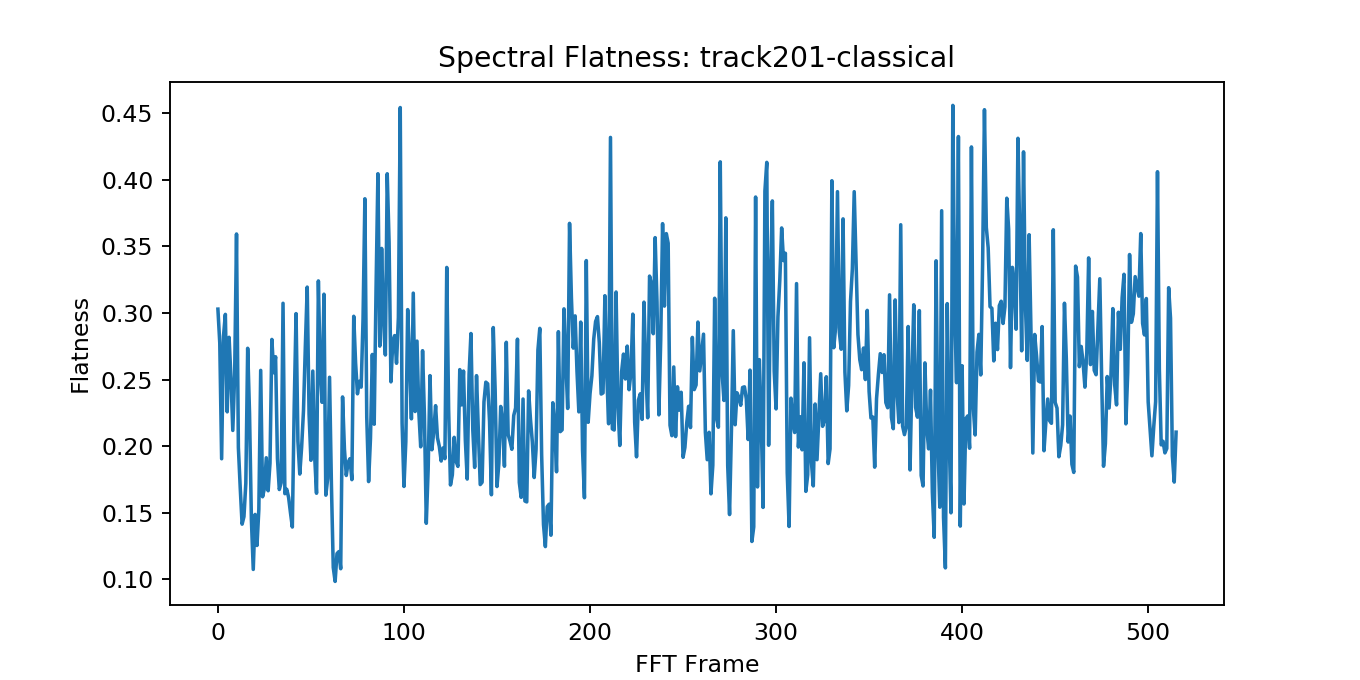
\includegraphics[width=0.9\textwidth]{flatness_track201-classical}
		\caption{Spectral flatness of 'track201-classical' as a function of frame number.}
		\label{fig:flatness_classical}
	\end{subfigure}
	\begin{subfigure}[t]{\hsize}
		\centering
		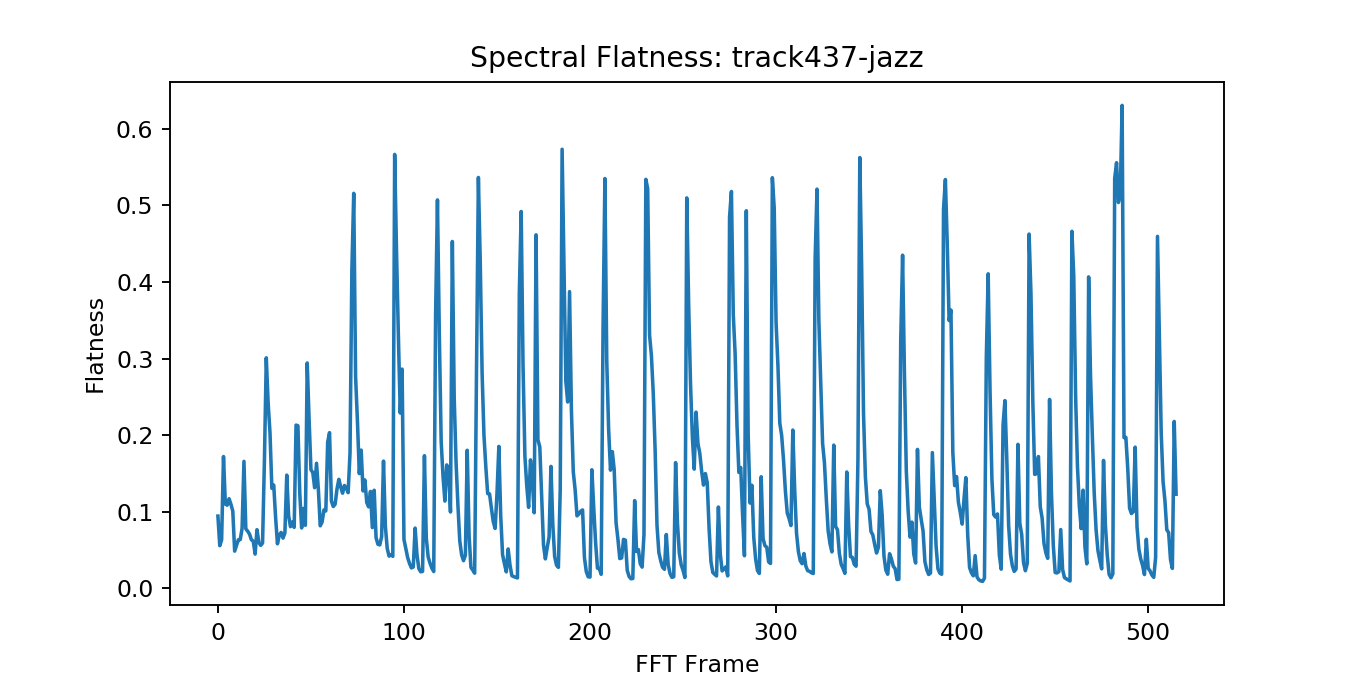
\includegraphics[width=0.9\textwidth]{flatness_track437-jazz}
		\caption{Spectral flatness of 'track437-jazz' as a function of frame number.}
		\label{fig:flatness_jazz}
	\end{subfigure}
	\caption{Flatness \label{fig:flatness}}
\end{figure}
\clearpage

\begin{figure}[tb]\ContinuedFloat
	\begin{subfigure}[t]{\hsize}
		\centering
		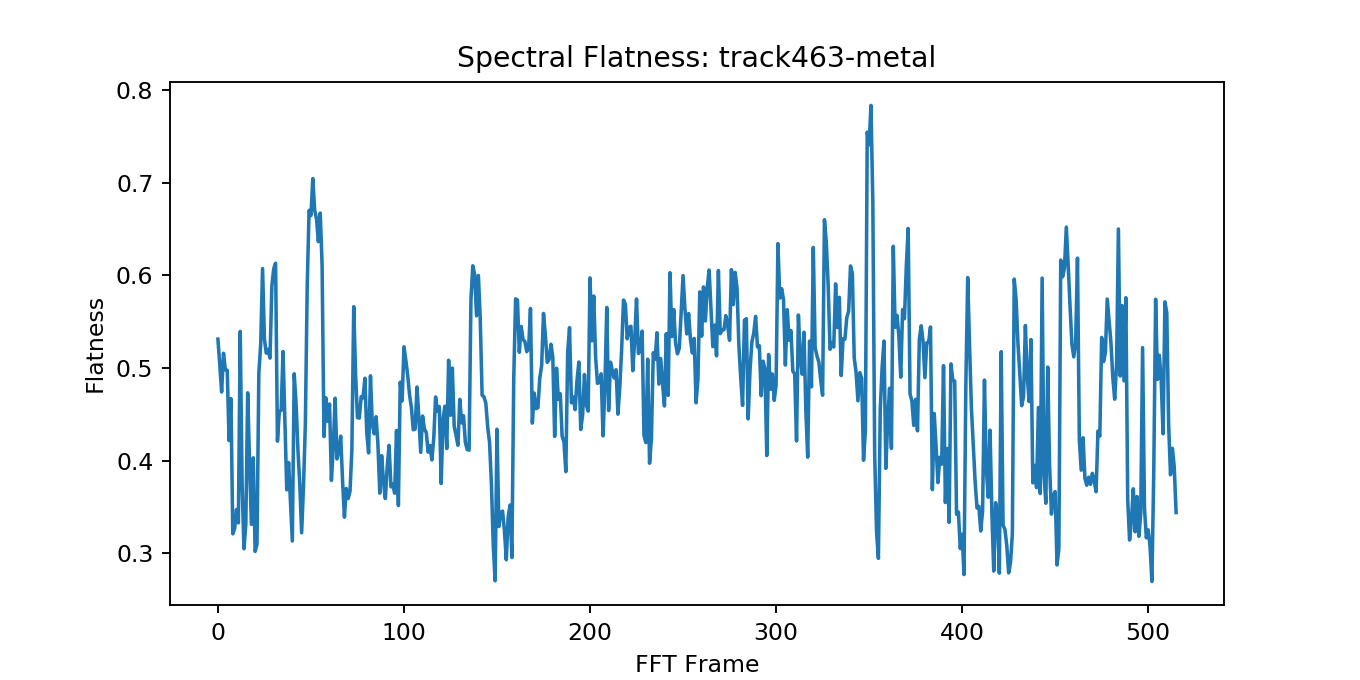
\includegraphics[width=0.9\textwidth]{flatness_track463-metal}
		\caption{Spectral flatness of 'track463-metal' as a function of frame number.}
		\label{fig:flatness_metal}
	\end{subfigure}
	\caption{Flatness}
\end{figure}

\paragraph{Comments} Notice the magnitude of flatness across the entire metal sample (figure \ref{fig:flatness_metal}) is almost double that of classical (figure \ref{fig:flatness_classical}). This is a direct indication that the metal track is much noisier. Then comparing the flatness curve of this jazz sample, we see the same alternating magnitudes as in the centroid (figure \ref{fig:centroid_jazz}) and spread (figure \ref{fig:spread_jazz}) curves, again indicating the noise inherent in the high-pitch components of this sample.

\subsection{Spectral Flux}
\paragraph*{} The spectral flux is a global measure of the spectral changes between two adjacent frames, $n-1$ and $n$,

\begin{equation} \label{eqn:F}
F_n = \sum_{k=0}^{K} (P_n(k)-P_{n-1}(k))^2
\end{equation}

Where $P_n(k)$ is the normalized frequency distribution for frame $n$, given by \ref{eqn:P}. Applying \ref{eqn:F} to the same three samples, the plots of figure \ref{fig:flux} were produced. See section \ref{app:flux} for Python implementation.

\begin{figure}[tb]
	\centering
	\begin{subfigure}[t]{\hsize}
		\centering
		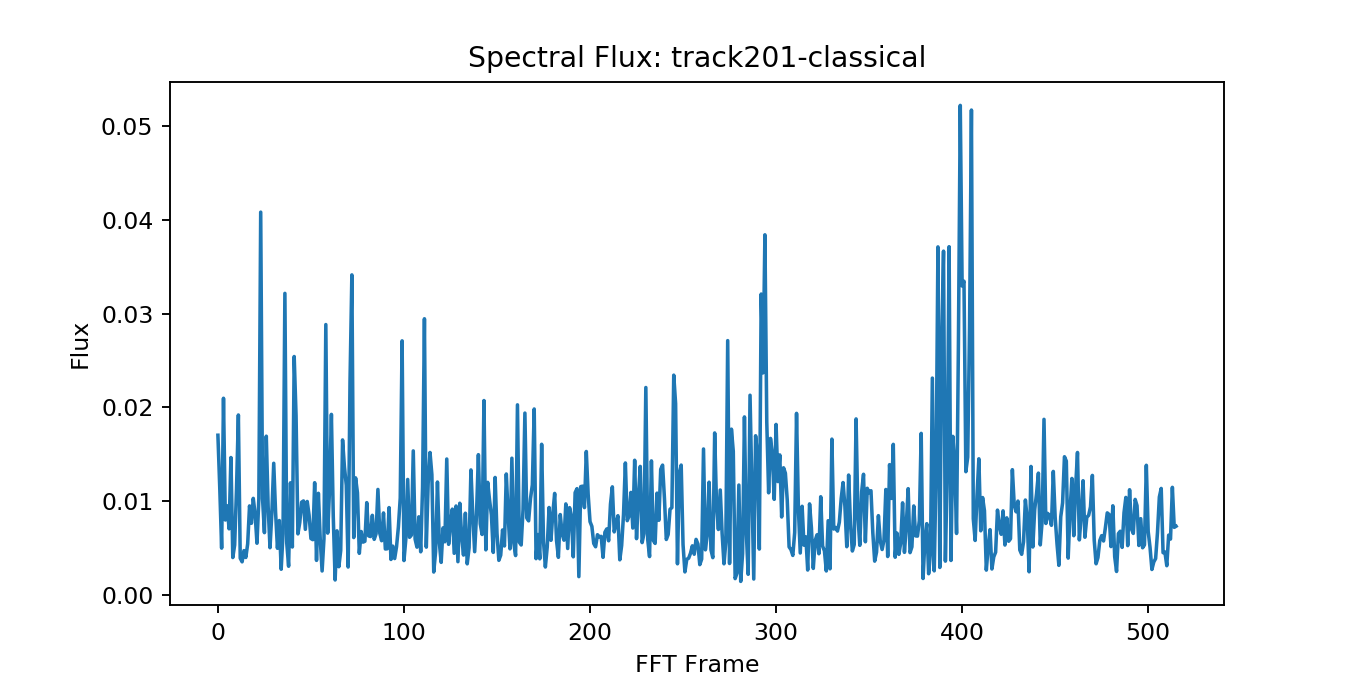
\includegraphics[width=0.9\textwidth]{flux_track201-classical}
		\caption{Spectral flux of 'track201-classical' as a function of frame number.}
		\label{fig:flux_classical}
	\end{subfigure}
	\begin{subfigure}[t]{\hsize}
		\centering
		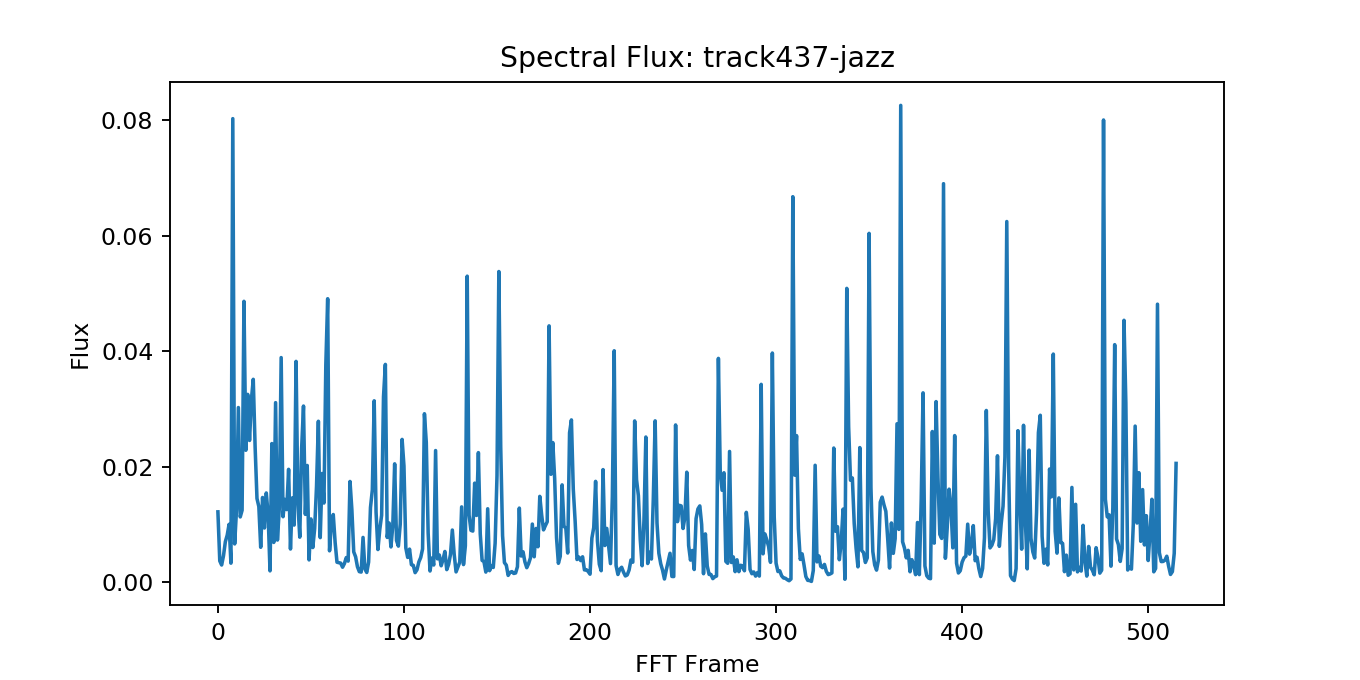
\includegraphics[width=0.9\textwidth]{flux_track437-jazz}
		\caption{Spectral flux of 'track437-jazz' as a function of frame number.}
		\label{fig:flux_jazz}
	\end{subfigure}
	\caption{Flux \label{fig:flux}}
\end{figure}
\clearpage

\begin{figure}[tb]\ContinuedFloat
	\begin{subfigure}[t]{\hsize}
		\centering
		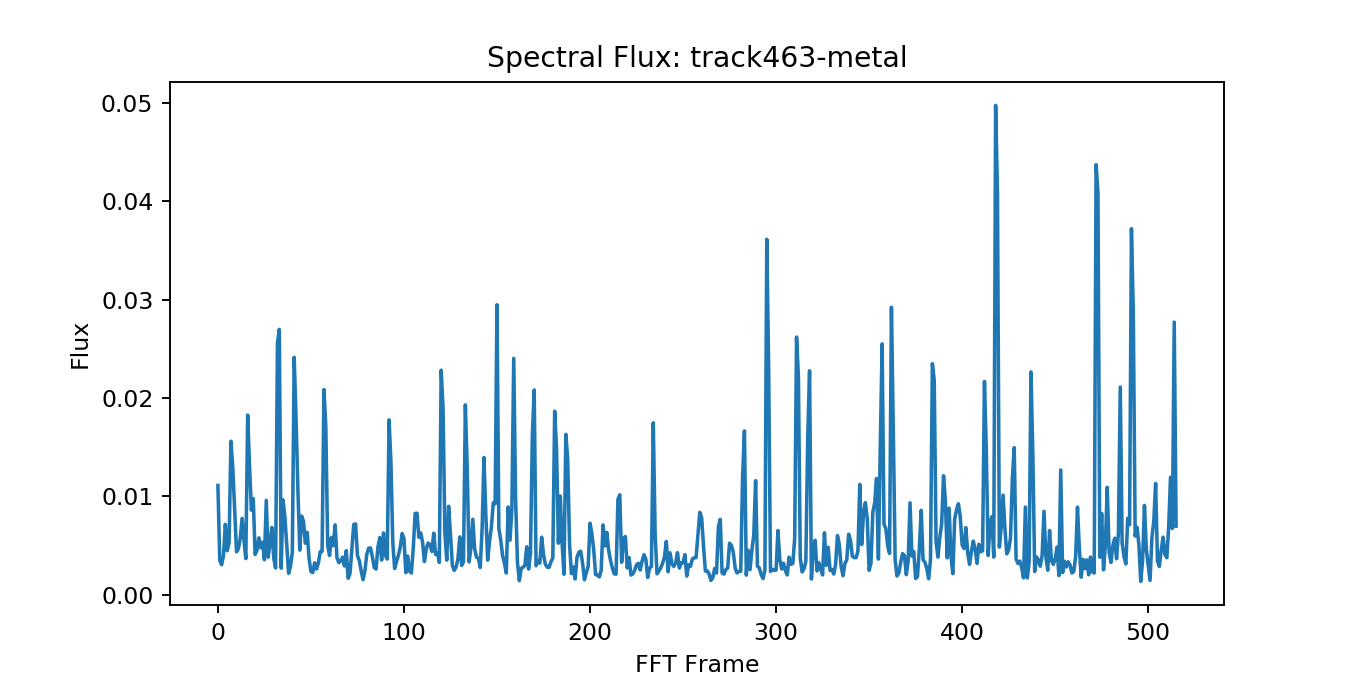
\includegraphics[width=0.9\textwidth]{flux_track463-metal}
		\caption{Spectral flux of 'track463-metal' as a function of frame number.}
		\label{fig:flux_metal}
	\end{subfigure}
	\caption{Flux}
\end{figure}

\paragraph{Comments} Considering the similarity of figures \ref{fig:flux_jazz} and \ref{fig:flux_metal}, spectral flux is not a good indication of genre. 

\section{Psychoacoustics}
\paragraph{Background} Psychoacoustics involves the study of the human auditory system and our perception of audio. In this lab, we will focus on some spectral content that can be defined mathematically. The human auditory system is sensitive to a range of frequencies with a logarithmic relationship. One very common model of human sound perception is called the mel/Bark scale.

\subsection{The mel/Bark Scale}
\paragraph*{} The Bark scale is defined as

\begin{equation*}
z = 7arcsinh(f/650)=7log\left(f/650+\sqrt{1+(f/650)^2}\right),
\end{equation*}

where $f$ is measured in Hz. However, in this lab, we will use a modified definition,

\begin{equation}
m = 1127.01048*log(1+f/700).
\end{equation}

\subsection{The Cochlear Filterbank}
\paragraph*{} Additionally, the human auditory system behaves like a sequence of filters (filterbank) with overlapping frequency responses.
Perception of pitch can be quantified using the total energy at the output of each filter, summing the spectral energy that falls into one critical band (the frequency band within which a second tone will interfere with the first). Our model is simple, with $N_B=40$ logarithmically spaced triangle filters centered at frequencies $\Omega_p$, which are implicitly defined as

\begin{equation}
mel_p = 1127.01048*log(1+\Omega_p/700).
\end{equation}

The set of frequencies chosen to correspond to each $\Omega_p$ is chosen to be equally spaced the the mel scale. Letting the indexing of the center frequencies of the filters start with $p=1$, we define

\begin{equation}
mel_p = p\frac{mel_{max}-mel_{min}}{N_B+1}+mel_{min}
\end{equation}

where $N_B$ is the number of filters in the filterbank and

\begin{align*}
mel_{min} &= 1127.01048*log(1+20/700), \\
mel_{max} &= 1127.01048*log(1+0.5*f_s/700),
\end{align*}

taking $f_s$ to be the sampling frequency of the audio. This definition gives $mel_{max}$ to be defined as the highest frequency preserved in the audio file and $mel_{min}$ to be $20Hz$ (a good baseline for the limit of human hearing).
We then define $H_p$, the hat filter corresponding to each filter to be centered around $\Omega_p$:

\begin{equation} \label{eqn:Hp}
H_p(f) = %
	\begin{dcases}
		\frac{2}{\Omega_{p+1}-\Omega_{p-1}}\frac{f-\Omega_{p-1}}{\Omega_p-\Omega_{p-1}} &\text{if $f \in [\Omega_{p-1},\Omega_p)$,} \\
		\frac{2}{\Omega_{p+1}-\Omega_{p-1}}\frac{\Omega_{p+1}-f}{\Omega_{p+1}-\Omega_{p}} &\text{if $f \in [\Omega_{p},\Omega_{p+1})$.}
	\end{dcases}
\end{equation}

Each triangular filter in \ref{eqn:Hp} is normalized such that the integral of each filter is 1 and the filters overlap so that the frequency where $H_p$ is maximum is at the starting frequency of the next filter, $H_{p+1}$ and ending frequency of $H_{p-1}$.

Finally, the implementation of the above derivation produces the plot shown in figure \ref{fig:mel}.

\begin{figure}
	\centering
	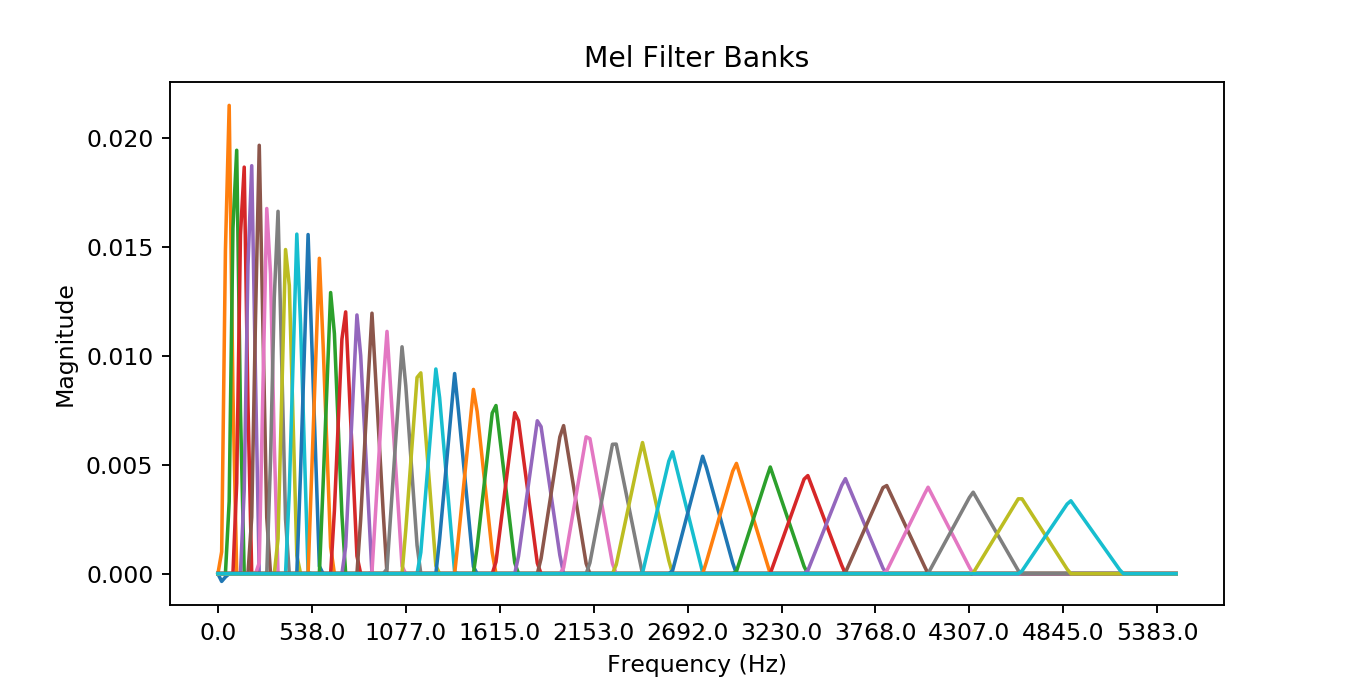
\includegraphics[width=0.9\textwidth]{melBanks}
	\caption{A collection of $N_B=40$ filterbanks to be used in the calculation of mfcc coeffients when convolved with an audio sample.}
	\label{fig:mel}
\end{figure}

\paragraph{Comments} The triangle filters in figure \ref{fig:mel} appear to decrease and increase on the left side of the x-axis, however this is an anomaly due to the quantization of values used to generate each filter. This can be seen in the offset peaks in a few of the filters. In reality, each filter maintains a unity integral over the range $N_B$. Python implementation for this can be found in section \ref{app:psycho}.

\pagebreak

\section{Conclusion} 
\paragraph*{} Spectral analysis of audio is definitively more useful than time-domain analysis, however this lab showed just how difficult it still can be to differentiate genres analytically. I think this was a good introduction to some of the useful statistical analysis techniques that can be used to programmatically sort signals based on characteristic features. Additionally, the script to run this analysis was relatively slow. With the digital age we live in, delay from input to output is very important, so some optimization would most likely help to make this sort of analysis even more useful. Next, I would like to apply this analysis to some of my favorite songs and see what I can gain from it. Eventually, I envision using this type of functionality to create a highly correlated audio visualizer or an advanced tool to equalize concert halls.

\pagebreak

\section{Appendix}

\subsection{Appendix A: Main} \label{app:main}
	\begin{lstlisting}[language=Python,label={lst:main}]
"""
Created on Wed Jan 16 15:24:09 2019

@author: Andrew Teta
"""

import scipy.io.wavfile
import scipy.signal
import scipy.stats
import numpy as np
import math
import matplotlib.pyplot as plt
from tkinter import filedialog

# UI dialog to select files -> selection of multiple files will run all functions for each file
files = filedialog.askopenfilenames()
# Loop over files selected
for f in files:
    filename = str.split(f,'/')[-1]
    filename = str.split(filename,'.')[0]
    filepath = f

    # Extract 24s sample from center of 60s clip
    fs,songSample = extractSample(filepath,24,60)

    # Calculate loudness (energy function returned just in case)
    E,sigma,Nloudness = loudness(songSample,512)

    # Save figures
    plt.figure(figsize=(8,4),dpi=170)
    plt.plot(range(Nloudness),sigma)
    plt.xlabel('FFT Frame')
    plt.ylabel('Loudness')
    plt.title('Loudness: '+filename)
    plt.savefig('figs/loudness_'+filename)
    plt.close()

    # Calculate zero-crossing-rate
    Z,Nzcr = zcr(songSample,512)

    plt.figure(figsize=(8,4),dpi=170)
    plt.plot(range(Nzcr),Z)
    plt.xlabel('FFT Frame')
    plt.ylabel('ZCR')
    plt.title('ZCR: '+filename)
    plt.savefig('figs/zcr_'+filename)
    plt.close()

    # Calculate spectrograms for Hann and Blackman windows
    spectroHann,spectroBlack,freqAxis,timeAxis = spectrogram(songSample,fs,512)
    spectroHann = np.transpose(spectroHann)
    spectroBlack = np.transpose(spectroBlack)

    mel = mfcc(spectroBlack,freqAxis,1,fs,40)

    # Generate frequencies axis labels
    tick = np.arange(0,len(freqAxis),25)
    label = np.around(tick*fs/512)

    # save figures
    plt.figure(figsize=(8,4),dpi=170)
    plt.imshow(spectroHann, cmap='inferno')
    plt.gca().invert_yaxis()
    plt.colorbar(shrink=0.5).set_label('Magnitude (dB)')
    plt.title('Hann Window Spectrogram: '+filename)
    plt.xlabel('FFT Frame')
    plt.ylabel('Frequency (Hz)')
    plt.yticks(tick,label)
    plt.savefig('figs/powerHann_'+filename)
    plt.close()

    plt.figure(figsize=(8,4),dpi=170)
    plt.imshow(spectroBlack, cmap='inferno')
    plt.gca().invert_yaxis()
    plt.colorbar(shrink=0.5).set_label('Magnitude (dB)')
    plt.title('Blackman Window Spectrogram: '+filename)
    plt.xlabel('FFT Frame')
    plt.ylabel('Frequency (Hz)')
    plt.yticks(tick,label)
    plt.savefig('figs/powerBlack_'+filename)
    plt.close()

    # calculate statistical vectors, centroid and spread
    centroid,spread,P,nFrames = spectralCentroid(songSample,fs,512)

    # save figures
    plt.figure(figsize=(8,4),dpi=170)
    plt.plot(centroid)
    plt.title('Spectral Centroid: '+filename)
    plt.ylabel('Frequency (Hz)')
    plt.xlabel('FFT Frame')
    plt.savefig('figs/centroid_'+filename)
    plt.close()

    plt.figure(figsize=(8,4),dpi=170)
    plt.plot(spread)
    plt.title('Spectral Spread: '+filename)
    plt.ylabel('Spread')
    plt.xlabel('FFT Frame')
    plt.savefig('figs/spread_'+filename)
    plt.close()

    # calculate spectral flatness
    flat,nFrames = flatness(songSample,fs,512)

    # save figure
    plt.figure(figsize=(8,4),dpi=170)
    plt.plot(flat)
    plt.ylabel('Flatness')
    plt.xlabel('FFT Frame')
    plt.title('Spectral Flatness: '+filename)
    plt.savefig('figs/flatness_'+filename)
    plt.close()

    sflux = flux(P)

    plt.figure(figsize=(8,4),dpi=170)
    plt.plot(sflux)
    plt.ylabel('Flux')
    plt.xlabel('FFT Frame')
    plt.title('Spectral Flux: '+filename)
    plt.savefig('figs/flux_'+filename)
    plt.close()

    print('done')
	\end{lstlisting}
	
\pagebreak

\subsection{Appendix B: Sample Extraction} \label{app:extractsample}
	\begin{lstlisting}[language=Python,label={lst:extractsample}]
# =============================================================================
# Input:
#   filepath = string containing absolute path to audio file
#   duration = length of sample to extract in seconds
#   location = start index of sample given in seconds
# Output:
#   arg1 = sampling frequency (Hz)
#   arg2 = sample of specified duration in seconds
# =============================================================================
def extractSample(filepath, duration, location):
    fs,data = scipy.io.wavfile.read(filepath)
    print('Read file: '+filepath+'\n')
    Tsample = 1/fs
    startIndex = int(location/Tsample)
    endIndex = startIndex + int(duration/Tsample)
    return fs,data[startIndex:endIndex]
	\end{lstlisting}

\subsection{Appendix C: Time-domain Analysis} \label{app:timedomain}
	\subsubsection{Loudness} \label{app:loudness}
		\begin{lstlisting}[language=Python,label={lst:loudness}]
# =============================================================================
# Input:
#   sample = audio clip
#   N = frame size
# Output:
#   arg1 = energy vector
#   arg2 = standard deviation vector
#   arg3 = num frames (for accurate plotting)
# =============================================================================
def loudness(sample,N):
    nframes = int(len(sample)/N)
    E = np.zeros(nframes)
    sigma = np.zeros(nframes)
    for n in range(nframes):
        E[n] = (1/N)*sum(sample[n*N:n*N+(N-1)])
    for n in range(nframes):
        sigma[n] = np.sqrt((1/N)*sum((sample[n*N:n*N+(N-1)] - E[n])**2))
    return E,sigma,nframes
		\end{lstlisting}
	\subsubsection{ZCR} \label{app:zcr}
		\begin{lstlisting}[language=Python,label={lst:zcr}]
# =============================================================================
# Input:
#   sample = audio clip
#   N = frame size
# Output:
#   arg1 = zero-crossing-rate
#   arg2 = num frames (for accurate plotting)
# =============================================================================
def zcr(sample,N):
    nframes = int(len(sample)/N)
    Z = np.zeros(nframes)
    for n in range(nframes):
        Z[n] = 1/(N-1) * sum(0.5*abs(np.sign(sample[n*N+1:n*N+(N-1)]) - np.sign(sample[n*N:n*N+(N-2)])))
    return Z, nframes
		\end{lstlisting}

\pagebreak

	\subsection{Appendix D: Frequency-domain Analysis} \label{app:frequencydomain}
		\subsubsection{Spectrogram} \label{app:spectrogram}
			\begin{lstlisting}[language=Python,label={lst:spectrogram}]
# =============================================================================
# Input:
#   sample = audio clip
#   fs = sampling frequency
#   N = frame size
# Output:
#   arg1 = spectrogram using Hann window
#   arg2 = spectrogram using Blackman window
#   arg3 = vector of axis points in frequency (Hz)
#   arg4 = vector of sxis points in time (s)
# =============================================================================
def spectrogram(sample,fs,N):
    # generate a Hann window
    wHann = scipy.signal.get_window('hann',N-1,False)
    # Generate Blackman window
    wBlack = scipy.signal.get_window('blackman',N-1,False)
    # Save figure
    plt.figure(dpi=170)
    plt.plot(wHann)
    plt.title('Hann Window')
    plt.xlabel('Samples')
    plt.ylabel('Magnitude')
    plt.savefig('figs/hann')
    plt.close()
    # save figure
    plt.figure(dpi=170)
    plt.plot(wBlack)
    plt.title('Blackman Window')
    plt.xlabel('Samples')
    plt.ylabel('Magnitude')
    plt.savefig('figs/blackman')
    plt.close()
    # Number of FFT frames
    nframes = int(len(sample)/N)
    SHann = np.zeros([nframes,int(N/2)])
    SBlack = np.zeros([nframes,int(N/2)])
    time = np.zeros(nframes)
    # Loop over FFT frames
    for n in range(nframes):
        # Calculate a frequency power spectrum for Hann window
        f,t,sH = np.transpose(scipy.signal.spectrogram(sample[n*N:n*N+(N-1)],fs,wHann,mode='magnitude'))
        # throw away values smaller than 10^-3 and square values
        sH = sH**2
        sH = np.where(sH < 10**-3, 10**-3, sH)
        # Repeat for Blackman window
        f,t,sB = np.transpose(scipy.signal.spectrogram(sample[n*N:n*N+(N-1)],fs,wBlack,mode='magnitude'))
        sB = sB**2
        sB = np.where(sB < 10**-3, 10**-3, sB)
        # Reshape a bit
        SHann[n,:] = np.transpose(sH*fs/N)
        SBlack[n,:] = np.transpose(sB*fs/N)
        time[n] = t
    # convert linear values to dB scale
    SHann = 20*np.log10(SHann/np.amax(SHann))
    SBlack = 20*np.log10(SBlack/np.amax(SBlack))
    return SHann,SBlack,f,time
			\end{lstlisting}
		\subsubsection{Spectral Centroid and Spread} \label{app:centroidspread}
			\begin{lstlisting}[language=Python,label={lst:centroidspread}]
# =============================================================================
# Input:
#   sample = audio clip
#   fs = sampling frequency
#   N = frame size
# Output:
#   arg1 = vector of size nframes of spectral centroids
#   arg2 = vector of size nframes of spectral spreads
#   arg3 = length of output vectors = nframes
# =============================================================================
def spectralCentroid(sample,fs,N):
    nframes = int(len(sample)/N)
    SP = np.zeros([nframes,int(N/2)])
    # Generate Blackman window
    wBlack = scipy.signal.get_window('blackman',N-1,False)
    # Generate a spectrogram matrix
    for n in range(nframes):
        f,t,sp = np.transpose(scipy.signal.spectrogram(sample[n*N:n*N+(N-1)],fs,wBlack,mode='magnitude'))
        SP[n,:] = np.transpose(sp)
    frange = np.shape(sp)[0]
    P = np.zeros([nframes,frange])
    mu = np.zeros(nframes)
    spread = np.zeros(nframes)
    # Loop over FFT frames
    for n in range(nframes):
        # calculate sum of all frequency components in this frame
        sfreq = sum(SP[n,0:frange])
        for k in range(frange):
            # calculate the relative 'probability' of each frequency bin
            P[n,k] = SP[n,k]/sfreq
            # calculate spectral centroid (center of mass) of each frame
            mu[n] = mu[n] + (k*fs/N)*P[n,k]
            # calculate spectral spread of each frame
            spread[n] = np.sqrt(spread[n] + P[n,k]*(k-mu[n])**2)
    return mu,spread,P,nframes
		\end{lstlisting}
		
\pagebreak
	\subsubsection{Spectral Flatness} \label{app:flatness}
		\begin{lstlisting}[language=Python,label={lst:flatness}]
# =============================================================================
# Input:
#   sample = audio clip
#   fs = sampling frequency
#   N = frame size
# Output:
#   arg1 = vector of length nframes of spectral flatness
#   arg2 = length of output vectors = nframes
# =============================================================================
def flatness(sample,fs,N):
    nframes = int(len(sample)/N)
    K = int(N/2)
    SP = np.zeros([nframes,int(N/2)])
    wBlack = scipy.signal.get_window('blackman',N-1,False)
    geo = np.zeros(nframes)
    arith = np.zeros(nframes)
    SF = np.zeros(nframes)
    for n in range(nframes):
        f,t,sp = np.transpose(scipy.signal.spectrogram(sample[n*N:n*N+(N-1)],fs,wBlack,mode='magnitude'))
        SP[n,:] = np.transpose(sp)
        geo[n] = scipy.stats.mstats.gmean(SP[n,:])
        arith[n] = np.mean(SP[n,:])
    SF = geo/arith
    return SF,nframes
		\end{lstlisting}
	\subsubsection{Spectral Flux} \label{app:flux}
		\begin{lstlisting}[language=Python,label={lst:flux}]
# =============================================================================
# Input:
#   P = probability matrix of dimension [nframes,N/2]
# Output:
#   arg1 = vector of length nframes of spectral flux
# =============================================================================
def flux(P):
    nframes = np.shape(P)[0]
    frange = np.shape(P)[1]
    F = np.zeros(nframes)
    for n in range(nframes):
        F[n] = sum((P[n,:]-P[n-1,:])**2)
    return F
		\end{lstlisting}
		
\pagebreak

\subsection{Psychoacoustics} \label{app:psycho}
	\subsubsection{Mel Filter Banks and Coefficients} \label{app:mfcc}
		\begin{lstlisting}[language=Python,label={lst:mfcc}]
# =============================================================================
# Input:
#   SP = audio sample spectrogram
#   f = list of frequency values with size = range of frequency bins in SP
#   n = frame index of SP
#   fs = sampling frequency of audio sample
#   nBanks = number of mel filter banks to generate
# Output:
#   arg1 = N_B x K (K = len(f)) matrix of filter values for H_p
#   arg2 = matrix of filter banks, size = nBnaks x len(f)
# =============================================================================
def mfcc(SP,f,n,fs,nBanks):
    mel_min = 1127.01048*math.log(1 + 20/700)
    omega_min = (math.e**(mel_min/1127.01048) - 1) * 700
    mel_max = 1127.01048 * math.log(1 + 0.5*fs/700)
    omega_max = (math.e**(mel_max/1127.01048) - 1) * 700
    # Generate frequency array in Hz
    linfreq = np.arange(np.round(omega_min,0),np.round(omega_max,0)+1,1)
    # Map frequency array to mel array
    melfreq = 1127.01048*np.log(1+linfreq/700)
    # Generate nbanks+2 mel frequencies uniformly spaced between mel_min and mel_max, inclusive
    mel = np.linspace(mel_min,mel_max,nBanks+2)
    # Array of center frequencies of each filter
    omega = np.zeros(nBanks+2,np.float64)
    # Populate array
    for i in range(nBanks+2):
        idx = np.argmin(np.abs(melfreq-mel[i]))
        omega[i] = linfreq[idx]
    # Generate filters
    nframes = np.shape(SP)[1]
    frange = np.shape(SP)[0]
    mfcc = np.zeros([nBanks,frange])
    h = np.zeros([nBanks,frange])
    plt.figure(figsize=(8,4),dpi=170)
    plt.ylabel('Magnitude')
    plt.xlabel('Frequency (Hz)')
    plt.title('Mel Filter Banks')
    tick = np.arange(0,len(f),25)
    label = np.around(tick*fs/512)
    plt.xticks(tick,label)
    for p in range(nBanks):
        omegaC = omega[p]
        omegaL = omega[p-1]
        omegaR = omega[p+1]
        for k in range(frange):
            freq = f[k]
            if (freq >= omegaL and freq < omegaC):
                h[p,k] = (2/(omegaR-omegaL)) * ((freq-omegaL)/(omegaC-omegaL))
            elif (freq >= omegaC and freq < omegaR):
                h[p,k] = (2/(omegaR-omegaL)) * ((omegaR-freq)/(omegaR-omegaC))
            else:
                pass
        plt.plot(range(len(f)),h[p])
    plt.savefig('figs/melBanks')
    #mfcc[p-1,:] = np.sum((np.abs(h*SP[:,n]))**2)
    return mfcc,h
		\end{lstlisting}
		
\pagebreak

\addcontentsline{toc}{section}{References}
\begin{thebibliography}{1}
\bibitem{convolution}
“Signals \& Systems.” Signals \& Systems, by Alan V. Oppenheim et al., The McGraw-Hill, 1997, p. 78.
%\bibitem{gibbs} 
%“Signals \& Systems.” Signals \& Systems, by Alan V. Oppenheim et al., The McGraw-Hill, 1997, pp. 218–219.

\end{thebibliography}

\end{document}

